% Chapter 3

\chapter{Bridges between Bayesian models and sparsity inducing norms}
\label{chapter:bayesian}
\noindent\makebox[\linewidth]{\rule{0.75\paperwidth}{0.4pt}}
\noindent\makebox[\linewidth]{\rule{0.75\paperwidth}{0.4pt}}

\localtableofcontents % local toc

\noindent\makebox[\linewidth]{\rule{0.75\paperwidth}{0.4pt}}
\noindent\makebox[\linewidth]{\rule{0.75\paperwidth}{0.4pt}}

\newpage
\vspace{1.5cm}
Parts of this chapter have been published in the following:
\begin{itemize}
\item \textbf{Y. Bekhti}, R. Badeau, and A. Gramfort, "Hyperparameter estimation in maximum a posteriori regression using group sparsity with an application to brain imaging," Signal Processing Conference (EUSIPCO), pp. 246-250, 2017.
\item \textbf{Y. Bekhti}, F. Lucka, J. Salmon, and A. Gramfort, "A hierarchical Bayesian perspective on majorization-minimization for non-convex sparse regression: application to M/\ac{eeg} source imaging," ArXiv preprint, (submitted).
\end{itemize}
\newpage

%----------Intro - general concepts --------------------------------------------------------
\section{Introduction - General concepts}
\label{sec:bayes_intro}
%%%%%%%%%%%%%%%%%%%%%%%%%%%%%%%%%%%%%%%%%%%%%%%%%%%%%%%%%%%%%%%%%%%%%%%%%%%%%%%

This chapter presents a different perspective on the MEG/EEG inverse problem. It tries to bridge the gap between two communities both interested in sparse models for solving inverse problems. As mentioned several times so far in this thesis, sparsity has emerged as a key concept to solve inverse problems, not only the MEG/EEG inverse problem, but also tomographic image reconstruction, deconvolution, or inpainting. The idea is also well established to regularize high dimensional regression problems in the field of machine learning. There are mainly two routes to introduce sparsity to such problems.

The first route, embraced by the optimization community and frequentist
statisticians, is to promote sparsity using convex optimization theory.
This line of work has led to now mature theoretical guarantees~\cite{FoRa13} when using regularization functions based on $\ell_1$ norm and other convex variants~\cite{Tibshirani96}. In particular, it has been popularized in the signal processing community under the name of compressed sensing~\cite{candes2008introduction} when combined with incoherent measurements.

There are however some limitations of sparsity promoting convex penalties based on the $\ell_1$ norm.
All the features (also called regressors, atoms or sources depending on the terminology of the community) involved in the solution form what is called the support of the solution.
Convex penalties can fail to identify the correct support in the presence of highly noisy data, but also in low noise setups if the forward operator (referred to as design matrix in statistics) is poorly conditioned. Convex regularizations also lead to a systematic underestimation bias in the amplitude of the coefficients~\cite{OsBuGoXuYi06,candes2008enhancing,chartrand2007exact,saab2008stable,ChHeSa17}.

To address these limitations of $\ell_1$-type models, reweighted schemes have been proposed~\cite{candes2008enhancing,Gasso,Rakotomamonjy,zhang2011sparse,strohmeier-etal:16}, of which the Adaptive \ac{lasso} \cite{Zou06} is the most commonly used in the statistics community: Starting from the Lasso estimator, which amounts to regressing with a standard $\ell_1$-norm as a regularizer (this estimator is sometimes referred to as Basis Pursuit Denoising (BPDN) \cite{Chen_Donoho_Saunders98} in signal processing), the Adaptive \ac{lasso} solves a sequence of weighted \ac{lasso} problems, where at each iteration the weights are chosen such that the strongest coefficients are less and less penalized.
From the optimization point of view, such an iterative scheme can be derived from so-called \ac{MM} strategies~\cite{lange2000optimization,schifano2010majorization}.
The idea behind MM is to minimize the objective function by successively minimizing upper bounds that are easier to optimize. Many well-known optimization approaches can be interpreted as instances of MM, \textit{\eg} simple gradient descent or proximal algorithms~\cite{Combettes2011}, expectation-maximization (EM)~\cite{Dempster77maximumlikelihood}, and difference-of-convex (DC) programming techniques~\cite{Horst:1999}.
%
More recently, re-weighted $\ell_1$-norm schemes based on \ac{MM} principle have been particularly popular to handle concave, hence non-convex regularizations such as $\ell_{0.5}$-quasi-norms or logarithmic functions. As such, these schemes are prone to converging to a local minimum determined by the initial, uniformly weighted $\ell_1$-norm solution (\textit{\ie} the \ac{lasso} estimator) that constitutes the first iterate. This first route has been defined in more details in Chapter~\ref{chapter:background} and Chapter~\ref{chapter:multiscale}.

The second route to introduce sparsity formulates the regression problem in a Bayesian framework and uses \ac{HBM} \cite{mackay2003information} for the inference.
The common way to formulate HBMs is to consider the variance parameters of Gaussian prior models as additional random variables which have to be estimated from the data as well. Their prior distributions are referred to as hyper-priors. Plausible solutions to the regression problem that both fit data and the \emph{a priori} assumption of sparsity are explicitly characterized as multiple distinct modes of the posterior distribution. This characterization is the Bayesian analogue to local minima in variational regression approaches when working with non-convex functionals. Different strategies to infer a point estimate for the parameters of interest from the \emph{a posteriori} distribution then lead to different algorithmic frameworks, for instance Variational Bayesian approaches~\cite{mackay2003information,jordan1999introduction,sato2004hierarchical,FrHaDaKiPhTrHeFlMa08,shervashidze2015learning}, \ac{SBL} approaches (also referred to as type-I or type-II maximum likelihood estimates) \cite{tipping2001sparse,wipf2004sparse,Wipf-Nagarajan:2009,zhang2011sparse} and fully-Bayesian strategies \cite{CaHaPuSo09,Lucka-etal:2012}.

This chapter focuses on the later one for a non-standard type of \ac{HBM} examined in \cite{Lu14} that combines a non-Gaussian prior with an $\ell_{1}$-type energy function with a specific Gamma hyper-prior.
For this \ac{HBM}, a simple alternating scheme to compute full maximum \emph{a posteriori} (MAP) estimates leads to exactly the same sequence of problems solved by \ac{MM} applied to $\ell_{1/2}$-type regularizations.
With this observation made, it is natural to revisit and improve these \ac{MM} schemes by leveraging the ability of the Bayesian framework to explore the modes of the posterior distribution by \ac{MCMC} schemes \cite{RoCa05,KaSo05}. This does not only mitigate the aforementioned initialization-dependence of \ac{MM}, but more importantly, it offers insights into the structure and importance of potentially multiple plausible sparse solutions. Yet, the benefit comes at the cost of additional computational efforts.

This chapter is organized as follows: First, it presents in a unified
perspective both routes to sparsity, \textit{\ie} reweighted $\ell_1$ MM schemes
and specific HBMs. We show that a particular optimization-based inference strategy recovers the MM algorithm. It then describes an \ac{HBM} inference strategy based upon an \ac{MCMC} sampling and shows on simulated and experimental MEG/EEG datasets how these stochastic \ac{MCMC}-based techniques do not only help to improve upon deterministic approaches but also help to reveal multiple plausible solutions to the inverse problem. This analysis leads to an \ac{UQ} of the support recovery of non-convex sparse regression problems that provides very useful complementary information, in particular for very ill-conditioned and under-determined applications like MEG/EEG source localization.

%----------Lp hypermodels ------------------------------------------------------------------
\section{Lp hyper-models}
In Bayesian statistics, a hyperprior is a prior distribution on a hyperparameter, that is, on a parameter of a prior distribution.
Firstly, the use of a hyperprior allows one to express uncertainty in a hyperparameter: taking a fixed prior is an assumption, varying a hyperparameter of the prior allows one to do sensitivity analysis on this assumption, and taking a distribution on this hyperparameter allows one to express uncertainty in this assumption: "assume that the prior is of this form (this parametric family), but that we are uncertain as to precisely what the values of the parameters should be"~\cite{bernardo2001bayesian}.

A popular choice of hyperprior is the gamma distribution with $\alpha$ and $\beta$ its corresponding parameters:
\begin{equation} \label{eq:gamma_dist}
	p(\lambda) = \frac{\beta^\alpha}{\Gamma(\alpha)}\lambda^{\alpha-1}\exp(-\beta\lambda)\mathbf{1}_{\RR^+}(\lambda), \; \lambda \in \RR
\end{equation}
where $\Gamma$ is the gamma function. In the following of this chapter, the hyperprior is always a gamma distribution.

%----------MAP estimation ------------------------------------------------------------------
%\section{MAP estimation}
%add a description about MAP and explain what is the bayes rule

%----------hyperparam estimation------------------------------------------------------------
\section{Hyperparameter estimation in the variational formulation}
%%% Intro from Hyperparam paper

%Before emphasizing the details of a full Bayesian formulation, 
This section investigates the estimation of the hyperparamter $\lambda$ in the variational formulation. One can notice that hyperparameter setting is a classical statistics problem for which a number of solutions have been proposed. In signal processing, the \ac{AIC} and \ac{BIC} criteria are quite popular techniques historically~\cite{schwarz1978estimating}. The SURE-based techniques~\cite{stein1981estimation} have also been quite popular and recently explored for denoising and compressed sensing applications~\cite{luisier2007new, guo2015near}. In a standard supervised machine learning setup with independent and identically distributed (i.i.d.) observations, \ac{CV} is the reference approach. 
Also, the Bayesian approach suited for probabilistic models offers a principled way to estimate hyperparameters using hyperpriors that introduce softer constraints than solutions with fixed parameter values. This benefit yet usually comes at a price in terms of computational cost. Finally, in a number of real scenarios, humans end up setting hyperparameters, as they can have some expert knowledge that can correct model mismatch.

In statistical machine learning, a hyperparameter typically aims at limiting overfitting by controlling the model complexity. In the particular case of regularized regression, classically a scalar parameter balances between the data fit and the penalty term. When using sparse regression, this parameter affects the sparsity of the solution, \emph{i.e.} how many covariates or regressors are used.

With \ac{CV}, some independent observations are left out of the inference and the
hyperparameter values that yield the best prediction performance on this data are selected. A search for the best parameter can be done with a time consuming exhaustive grid-search, smooth optimization (see \cite{pedregosa2016hyperparameter} and references therein), sequential or even random search~\cite{bergstra2011algorithms, bergstra2012random}. The \ac{CV} approach however needs the i.i.d. assumption to be fulfilled, which is not always the case in practice, e.g. when working with signals or arrays of sensors as in the case of our application to brain imaging.

To keep it as a hierarchical Bayesian model problem and following a recent paper of Pereyra~\cite{Figueiredo}, we consider a \ac{HBM} and propose to use a \ac{MAP} estimation for the hyperparameters.

This thesis is particularly interested in the high-dimensional regression setting using Group-\ac{lasso}-like structured sparsity as seen so far. In the literature a number of approaches have been proposed and MAP estimates that boil down to penalized regression with smooth or non-smooth penalties are the standard approaches employed by neuroscientists~\cite{haufe2008combining,ou2009distributed, bolstad2009space, wipf2009unified,gramfort2012mixed,lucka2012hierarchical,valdes2009eeg}.

In a variational formulation, the value of the hyperparameter $\lambda$ depends on the problem at hand, the noise level, and on the choice of regularization $\mathcal{P}(\mathbf{X})$.
Finding a way to estimate the hyperparameter with minimal user intervention is therefore particularly important, as it makes a comparison between different models and regularization easier.

Recently \textit{Pereyra et al.} \cite{Figueiredo} proposed a strategy for hyperparameter estimation in the context of MAP inference when the prior or the regularizer is a $k$-homogeneous function. The regularizer $\mathcal{P}$ is a $k$-homogeneous function if there exists $k\in\RR^+$ such that:\\
\begin{center}
 $\mathcal{P}(\eta \mathbf{X}) = \eta^k\mathcal{P}(\mathbf{X}),
 \hspace{6pt} \forall \mathbf{X}\in\RR^{S\times T}$  \hspace{4pt} and \hspace{4pt}  $\forall \eta > 0$.
 \end{center}

The $k$-homogeneous condition is satisfied for all $\ell_{p,q}$ mixed norms. We focus on the estimation of the hyperparameters for hierarchical Bayesian models yielding convex $\ell_{2,1}$ ($\mathcal{P}(\mathbf{X})=\|\mathbf{X}\|_{2,1}$) or non-convex $\ell_{2,0.5}$ penalties, which are respectively $1$-homogeneous and $0.5$-homogeneous. The non-convex penalization is solved using iterative re-weighted convex optimization schemes, \textit{i.e.} each iteration is a weighted $\ell_{2,1}$-norm as described in Section~\ref{section:MM}.

In \cite{Figueiredo}, the fixed point strategy proposed is validated on an image denoising problem using an analysis prior, \textit{i.e.} where the solution is not sparse but has a sparse representation in some transformed domain. This section illustrates and explains why the method from~\cite{Figueiredo} cannot be used out-of-the-box when using a synthesis prior for an under-determined problem. A synthesis prior is when the solution itself is sparse.

\subsection{Hierarchical Bayesian modeling and reformulation}

% Bayesian modeling imposes hyperpriors, which are priors on the distributions of the hyperparameters. Here we chose gamma distribution as defined in Equation~\eqref{eq:gamma_dist}.

The result shown in~\cite{Figueiredo} and adapted to our problem and the notations used in this manuscript is the following. Using a joint MAP estimator of $\lambda$ and $\mathbf{X}$, it states that $\hat{\lambda}$ should satisfy:
\begin{equation} \label{eq4}
	\hat{\lambda} = \frac{ST/k + \alpha - 1}{\mathcal{P}(\mathbf{\hat{X}}_{\hat{\lambda}}) + \beta} \enspace ,
\end{equation}
where $\mathbf{\hat{X}}_{\hat{\lambda}}$ is the solution of Equation~\eqref{eq_reg} (page~\pageref{eq_reg}) for $\lambda = \hat{\lambda}$. In \cite{Figueiredo}, it is further suggested to set $\alpha$ and $\beta$ to 1.

Looking at Equation~\eqref{eq4}, one can observe that if $ST$ is big, which is the case for high dimensional problems, the numerator can significantly dominate the denominator, especially if the estimate $\hat{X}$ is very sparse.
In practice using Equation~\eqref{eq4} in this scenario results rapidly in huge values of $\lambda$ and empty supports. This issue is much less critical when using an analysis prior for denoising as in~\cite{Figueiredo}, as the size of the unknown coefficients is in this case $NT$, where $NT \ll ST$.\\

As reported earlier, the update of the regularization parameter $\lambda$ as in (Equation~\eqref{eq4}) is not suitable for the synthesis prior $\mathcal{P}(\mathbf{X})$. The issue is due to the over-scaled numerator compared to the denominator. When the problem is important (as in~\cite{Figueiredo}) - $ST$ is big, whereas the support in $\mathbf{X}^\star$ is small - the estimated parameter $\lambda$ then explodes, resulting in an empty support.

To overcome this problem, we propose to rewrite the objective function in such a way that we obtain the same solution $\mathbf{X}$ but with a multiplicative factor $\frac{\lambda}{ST}$. The new equivalent formulation can be written as:
\begin{equation} \label{eq5}
    \mathbf{\hat{X}} = \argmin_{\mathbf{X}} \frac{ST}{2}\|\mathbf{M - GX}\|^2_{Fro} + \lambda\mathcal{P}(\mathbf{X})
\end{equation}

Note that this is just a reparametrization of Equation~\eqref{eq_reg}. In practice, this boils down to multiplying $\mathbf{M}$ and $\mathbf{G}$ by $\sqrt{ST}$. However this only solves one difficulty in the parameter's update. Another disadvantage is that none of the parameters in Equation~\eqref{eq4} takes into account the scale of $\mathbf{G}$. The next section explains how to use results from convex optimization to properly calibrate the hyperprior parameters $\alpha$ and $\beta$ given $\mathbf{M}$, $\mathbf{G}$ and $\mathcal{P}$.

\subsection{Setting hyperpriors with a single hyperparameter}
As in~\cite{Figueiredo}, Gamma hyperpriors are used to derive two iterative algorithms that simultaneously estimate a single hyperparameter $\lambda$ and the entries of $\mathbf{X}$, yet the values of $\alpha$ and $\beta$ are still to be defined.
In~\cite{Figueiredo}, it is suggested to set $\alpha$ and $\beta$ to 1, which turns out to be inappropriate for underdetermined inverse (deconvolution) problems as our MEG/EEG brain imaging problem of interest.\\

A first observation is that $\alpha$ and $\beta$ should default to reasonable values and be insensitive to trivial changes in matrix $\mathbf{G}$ such as scaling, \textit{i.e.} multiplying $\mathbf{G}$ by a scalar. This is the problem we investigate now.

In Equation~\eqref{eq4}, the numerator would not be affected by a rescaling of $\mathbf{G}$. However, the denominator that contains $\mathcal{P}(\mathbf{X}_{\lambda^\star})$ would. To make the estimation robust to changes of $\mathbf{G}$ such as scaling, one therefore needs to modify the numerator, hence make $\alpha$ a function of $\mathbf{G}$. Setting $\alpha$ to 1 independently of the problem, as in~\cite{Figueiredo}, is certainly inadequate.

In order to set the value of $\alpha$, we propose to take advantage of the fact that if $\mathcal{P}(\mathbf{X})=\|\mathbf{X}\|_{2,1}$, one can analytically compute $\lambda_{max}$, which is defined as the smallest regularization parameter for which the solution is zero~\cite{bach2012optimization}. It is given by:
\begin{equation}
\lambda_{max} = \|\mathbf{G}^\top\mathbf{M}\|_{2,\infty}=\max_i \|(\mathbf{G}^\top\mathbf{M})[i, :]\|_2.
\end{equation}
Parameter $\lambda$ can therefore be parametrized as a fraction, or a percentage, of $\lambda_{max}$.
This allows us to have a good a priori guess on the peak of the gamma distribution. We set the peak, \textit{a.k.a.} the mode, to $mode=\tau\times\lambda_{max}$, with $\tau\in[0,1]$.
\\

Once the mode is known, it is straightforward to fix the value of $\alpha$: $mode =\frac{\alpha - 1}{\beta}$ for $\alpha \ge 1$. From now on we fix $\alpha$ as:

\begin{equation}
\alpha = mode \times \beta + 1 = \tau\times \lambda_{max} \times \beta + 1 \enspace .
\end{equation}

Concerning the parameter $\beta$, for our specific MEG/EEG problem of interest we fix it so that $99\%$ of the probability density of the gamma distribution is between $20\%$ and $70\%$ of $\lambda_{max}$. This is motivated by the fact that in our case solutions are expected to be extremely sparse, with only a handful of active brain regions. This is of course application specific.
 
\subsection{Estimation of a vector of hyperparameters}

The penalizations of the form $\mathcal{P}(\mathbf{X})=\|\mathbf{X}\|_{2,\cdot}$ are separable in $S$ groups of coefficients.
As only a few groups are expected to be active, a natural idea is to penalize less the important groups. To do this, we propose to estimate one parameter per group of coefficients or row of $\mathbf{X}$ using the convex $\ell_{2,1}$ penalization. Let us now derive a result similar to Equation~\eqref{eq4} but in the more general case of one $\lambda$ per group.

Rewriting Equation~\eqref{eq_reg} in the MAP framework leads to: 
\begin{equation}
\mathbf{X}^\star = \argmax_{\mathbf{X}}
p(\mathbf{X}, \mathbf{M}|\lambda) = \argmax_{\mathbf{X}} p(\mathbf{M}|\mathbf{X})p(\mathbf{X}|\lambda) 
\end{equation}
where $p(\mathbf{M}|\mathbf{X})$ is the likelihood function corresponding to the first term in Equation~\eqref{eq_reg} and $p(\mathbf{X|\lambda})$ is the regularization corresponding to the second term in Equation~\eqref{eq_reg}. This Bayesian formulation requires to compute the normalization factor $C(\lambda)$ in $p(\mathbf{X}|\lambda)=\exp(-\lambda\mathcal{P}(\mathbf{X}))/C(\lambda)$. Computing this constant $C(\lambda)$ in general is intractable as it involves an integration. Yet~\cite{Figueiredo} showed that it admits an exact closed-form when the penalization is $k$-homogeneous as $C(\lambda)=D\lambda^{-ST/k}$ where $D=C(1)$ is a constant independent of $\lambda$~\cite{Figueiredo}.\\

We now propose a joint-MAP estimation with $\lambda\in\RR^S$.
% A natural extension to \eqref{eq2} to the case of an unknown vector $\lambda$ is to compute a joint MAP estimator as in \cite{Figueiredo}.
We look for $(\mathbf{X}^\star, \lambda^\star) \in\RR^{(S\times T)} \times \RR^{S}$ which maximizes $p(\mathbf{X}, \lambda|\mathbf{M})$. A sufficient condition of optimality is given by:
\begin{equation} \label{eq7}
(0_{(S\times T)}, 0_{S}) \in -\partial_{\mathbf{X},\lambda} \log p(\mathbf{X^\star}, \lambda^\star|\mathbf{M})
\end{equation}

\textit{i.e.}
\begin{equation} \label{eq8}
\begin{aligned}
0_{S\times T} \in -\partial_{\mathbf{X}} \log p(\mathbf{X^\star}, \lambda^\star|\mathbf{M}), \hspace{9mm} \\
%0_{S} \in \partial_{\lambda} -\log p(\mathbf{X^\star}, \lambda^\star|\mathbf{M}),
0 \in -\partial_{\lambda_i} \log p(\mathbf{\mathbf{X}^\star}, \lambda^\star|\mathbf{M}) \hspace{6mm} \forall i,
\end{aligned}
\end{equation}
where $\partial_{\mathbf{X},\mathbf{\lambda}}$ is the set of subgradients (the subdifferential).\\

The optimization over $\mathbf{X}$ at iteration $k$ satisfies Equation~\eqref{eq5}: %if we choose $\lambda=\lambda^\star$.
\begin{equation*}	
\mathbf{X}^{(k)}=\argmin_{\mathbf{X}\in\RR^{S\times T}} \frac{ST}{2}\|\mathbf{M}-\mathbf{GX}\|_{Fro}^2 + \sum_{i} \mathbf{\lambda}[i]^{(k-1)}\|\mathbf{X}[i,:]\|.
\end{equation*}
The next step is to optimize over $\lambda_i, \forall i$. Equation~\eqref{eq8} leads to:
\begin{equation} \label{optimlambda}
0\in -\partial_{\mathbf{\lambda}[i]} \log p(\mathbf{X}^{(k)},\mathbf{M}|\mathbf{\lambda}) -\partial_{\mathbf{\lambda}[i]} \log p(\mathbf{\lambda}).
\end{equation} 

Using $p(\mathbf{X}^{(k)},\mathbf{M}|\mathbf{\lambda})=p(\mathbf{M}|\mathbf{X}^{(k)})p(\mathbf{X}^{(k)}|\mathbf{\lambda})$, one has that:
\begin{equation}
-\partial_{\mathbf{\lambda}[i]} \log p(\mathbf{X}^{(k)}, \mathbf{M}|\mathbf{\lambda}) = -\partial_{\mathbf{\lambda}[i]} \log p(\mathbf{X}^{(k)}|\mathbf{\lambda}).
\end{equation}

We then use the normalization factor $C(\mathbf{\lambda})$ which gives:\\
\begin{equation}
 - \partial_{\mathbf{\lambda}[i]} \log p(\mathbf{X}^{(k)}, \mathbf{M}|\mathbf{\lambda})=\|\mathbf{X}[i,:]\| + \partial_{\mathbf{\lambda}[i]} \log C(\mathbf{\lambda})
\end{equation}
 and 
\begin{equation} 
 \partial_{\mathbf{\lambda}[i]} \log C(\mathbf{\lambda})=\frac{-ST}{k\mathbf{\lambda}[i]}.
\end{equation}
  Regarding the second term in Equation~\eqref{optimlambda}, Equation~\eqref{eq:gamma_dist} yields $-\partial_{\lambda_i} \log p(\lambda) = -\frac{\alpha-1}{\lambda_i} + \beta$.
Completing the derivations, the equation for each $\lambda_i$, $i\in[1\dots S]$, reads:
\begin{equation} \label{eq9}
\lambda^\star_i=\frac{ST/k + \alpha - 1}{\|X_{\lambda^\star}[i,:]\| + \beta} \enspace .
\end{equation}

\subsection{Experiments}
\subsubsection{Simulation study}

We generated a simulation dataset with $N=302$ sensors, $T=190$ time samples and $S=1500$ sources. Four sources were randomly selected to be active with realistic waveforms obtained from the MIND dataset~\cite{weisend2007paving}. The linear forward operator $\mathbf{G}$ was a random matrix, whose columns were normalized to 1. Two levels of white noise were added to the simulation. We always used $\tau=0.5$.

\begin{figure}
	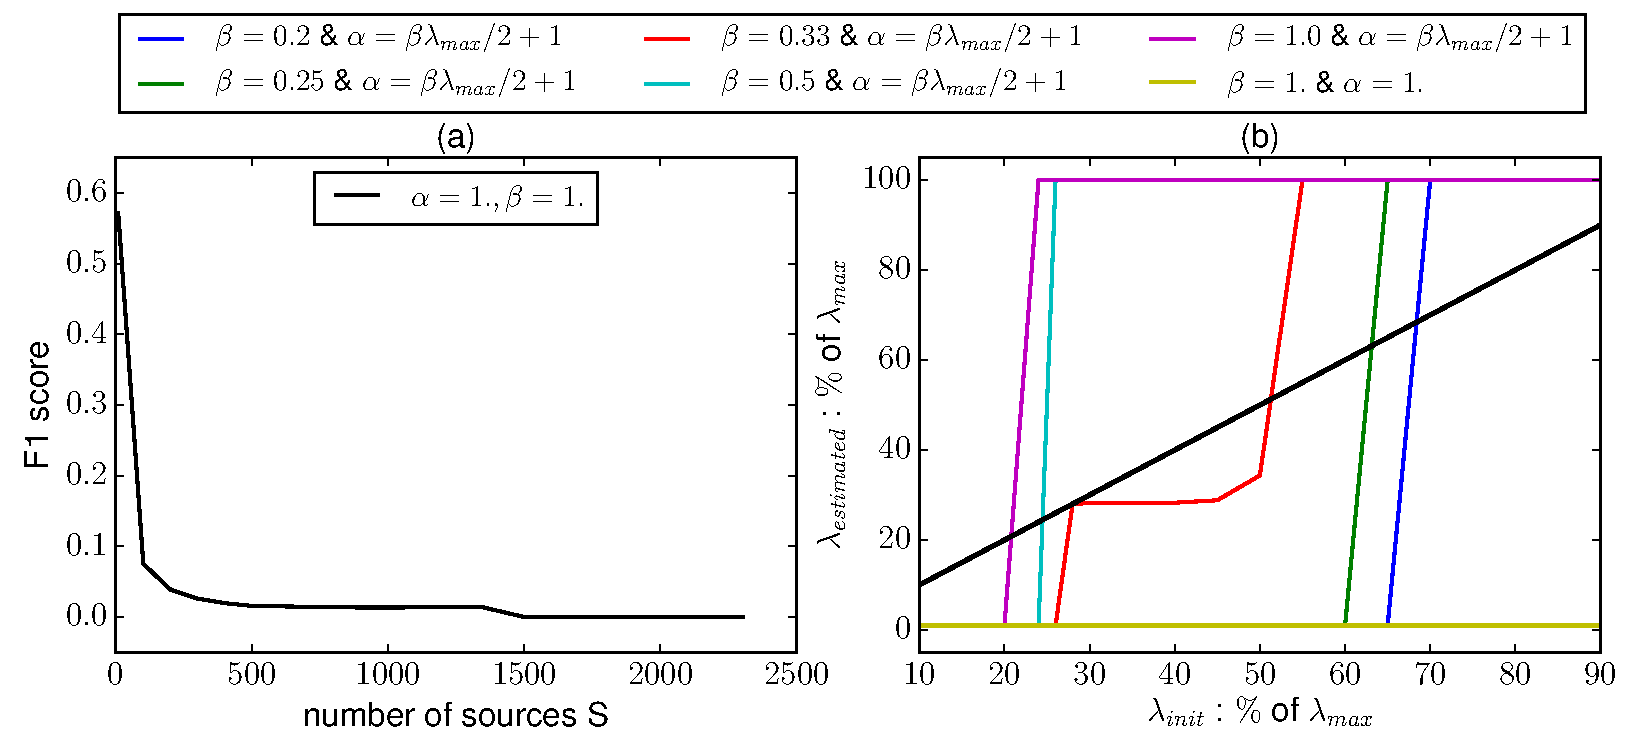
\includegraphics[width=0.95\textwidth]{hyperparam_estim/fig1_eusipco_data_size_and_fix_points_a_b}
    \caption{(a) Source identification results for different numbers of sources measured with F1 score using $\alpha=1$ and $\beta=1$. The higher the number of regressors, the worse the performance is. (b) Estimated $\lambda$ as a function of $\lambda_{init}$ for different values of $a$ and $b$. The red curve for $\beta=0.33$ gives the best plateau, which demonstrates that $(a,b)$ shall be carefully adjusted.}
    \label{fig:fig1_eusipco}
\end{figure}

In order to illustrate the issue when using a synthesis prior for large problems, we run the estimation of the hyperparameter $\lambda$ as suggested in~\cite{Figueiredo} using the $0.5$-homogeneous non-convex prior. Figure~\ref{fig:fig1_eusipco}-(a) shows the F1 score \footnote{The $F_1$ score is the harmonic mean of precision and recall: $F_1=2.\frac{precision . recall}{precision + recall}$} of the source reconstruction (1 for good reconstruction and 0 for bad). The source estimation is failing for almost all the range of data size. Figure~\ref{fig:fig1_eusipco}-(b) shows the results after reformulating the problem with different settings of $\alpha$ and $\beta$. One can notice that a setting as in~\cite{Figueiredo} with $\alpha=1$ and $\beta=1$ always gives an estimated $\lambda$ around $1\%$ of $\lambda_{max}$, which is not promoting the sparsity we are looking for in this kind of setting. For this aim, we varied the values of $\beta$ and computed $\alpha$ as defined before. Figure~\ref{fig:fig1_eusipco}-(b) shows that for most values of $\beta$ we have rather a too low estimation of $\lambda\approx 1\%$ or a too high $\lambda\geq 100\%$ resulting in zero source found active. Interestingly, setting $\beta=1/3$ gives a plateau at $\hat{\lambda}$ close to $0.3\lambda_{max}$. This is an evidence of a clear fixed point for the iterative process $\lambda^{(t+1)}=f(\lambda^{(t)})$, where $f$ is the update rule of $\lambda$ in Equation~\eqref{eq4}. We use $\beta=1/3$ from now on and its corresponding $\alpha$.

Figure~\ref{fig:mxne_vs_irmxne} represents the simulated sources with stars and the estimated ones with plain lines. Figure~\ref{fig:mxne_vs_irmxne}-(a)-(b) display results with the $\ell_{2,1}$ and $\ell_{2,0.5}$ norms respectively, using one hyperparameter initialized to $\lambda=0.5\lambda_{max}$. One can see that in Figure~\ref{fig:mxne_vs_irmxne}-(a), the $\ell_{2,1}$ norm recovers the four sources with an amplitude bias (the estimated amplitude is lower than the exact one), and that several sources shown in light green are almost flat around zero but still found as active sources. There is no way to reduce the support without losing one of the four simulated sources, \textit{i.e.} the $\ell_{2,1}$ norm with one hyperparameter fails to recover the exact simulated sources.\\
The $\ell_{2,0.5}$ norm in (b) estimates the exact four source amplitudes without amplitude bias thanks to the non-convexity~\cite{strohmeier-etal:16}. On the other hand, Figure~\ref{fig:mxne_vs_irmxne}-(c) shows the results for the convex penalty using one hyperparameter per source. It can be seen that it is qualitatively equivalent to the non-convex penalty. \\

\begin{figure}
	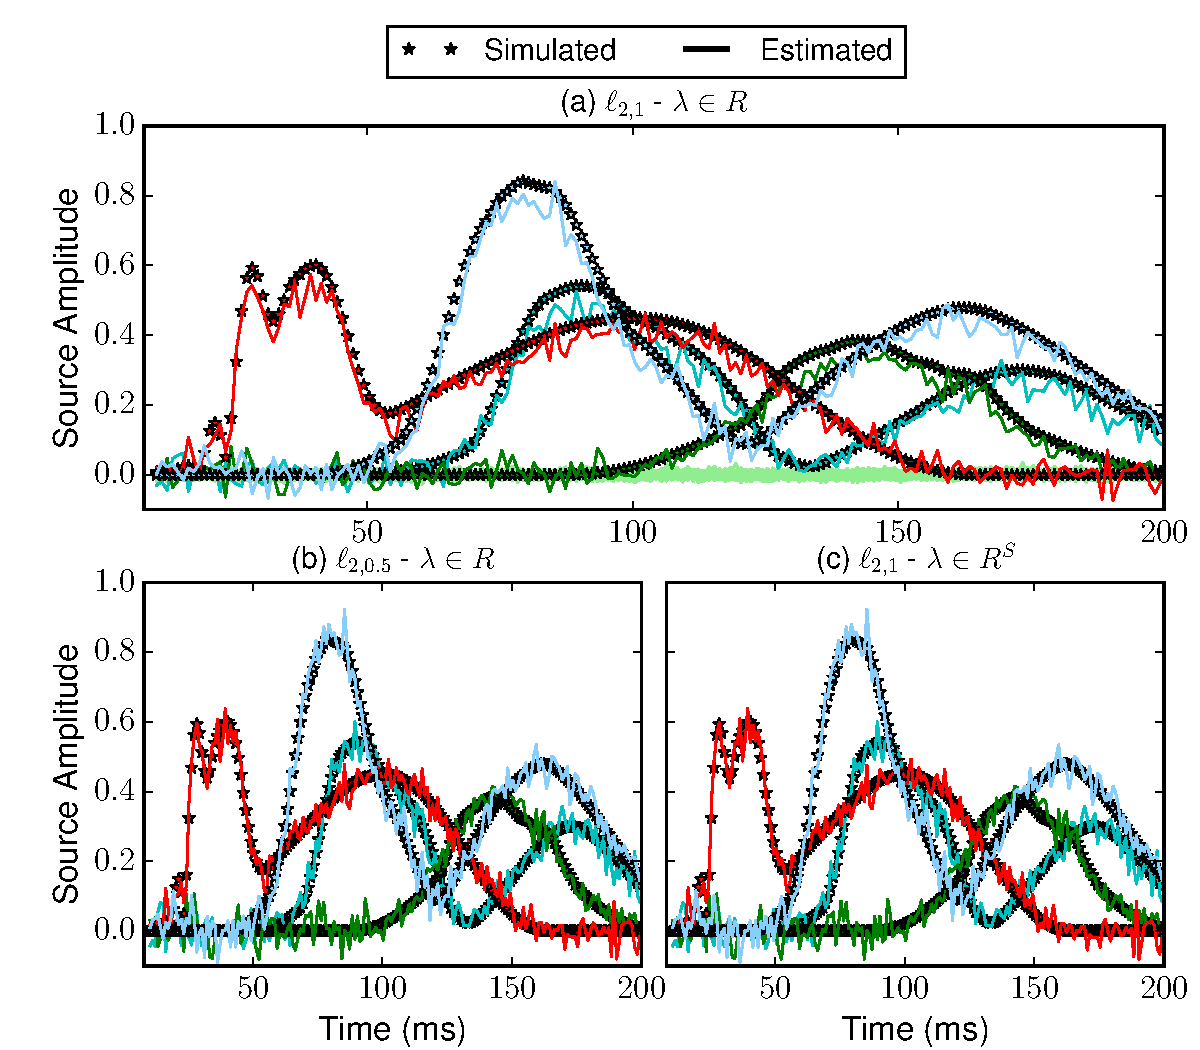
\includegraphics[width=0.95\textwidth]{hyperparam_estim/mxne_vs_irmxne}
    \caption{Source reconstruction on simulated data. (a): Source estimates obtained using $\ell_{2,1}$ with one $\lambda$. The solution is not sparse enough (zero sources in light green) and there is an amplitude bias between the exact amplitudes (stars) and the estimated ones (raw lines). (b): Good reconstruction of the four sources using $\ell_{2,0.5}$ and one $\lambda$, which is equivalent to the reconstruction using the $\ell_{2,1}$ norm with $\lambda\in\RR^S$ (c). Each of the four sources is encoded with a different color.
    }
    \label{fig:mxne_vs_irmxne}
\end{figure}

The advantage of having one hyperparameter per source is to pick up only the sources involved in the measurement $\mathbf{M}$ and drop the extra almost-zero sources visible in Figure~\ref{fig:mxne_vs_irmxne}-(a) (light green). This extension produces sparser results and less amplitude bias without casting the problem as non-convex. This figure also suggests a link between the non-convex prior and one hyperparameter per source. As the non-convex prior is an iterative procedure estimating an internal weight to produce a better solution, the fact to have one hyperparameter per source can also be seen as a weight to define better source estimates. A more accurate study of this can be found in the next section~\ref{link_hbm_mm}.


\subsubsection{Experimental results with MEG auditory data}

We applied the estimation of a single hyperparameter and a hyperparameter per source using the convex $\ell_{2,1}$ penalty on a real open dataset (MNE sample dataset \cite{mne}). It corresponds to a dataset with $N=305$ sensors, $T=55$ time samples and $S=7498$ sources. 
\begin{figure}
%\begin{center}	
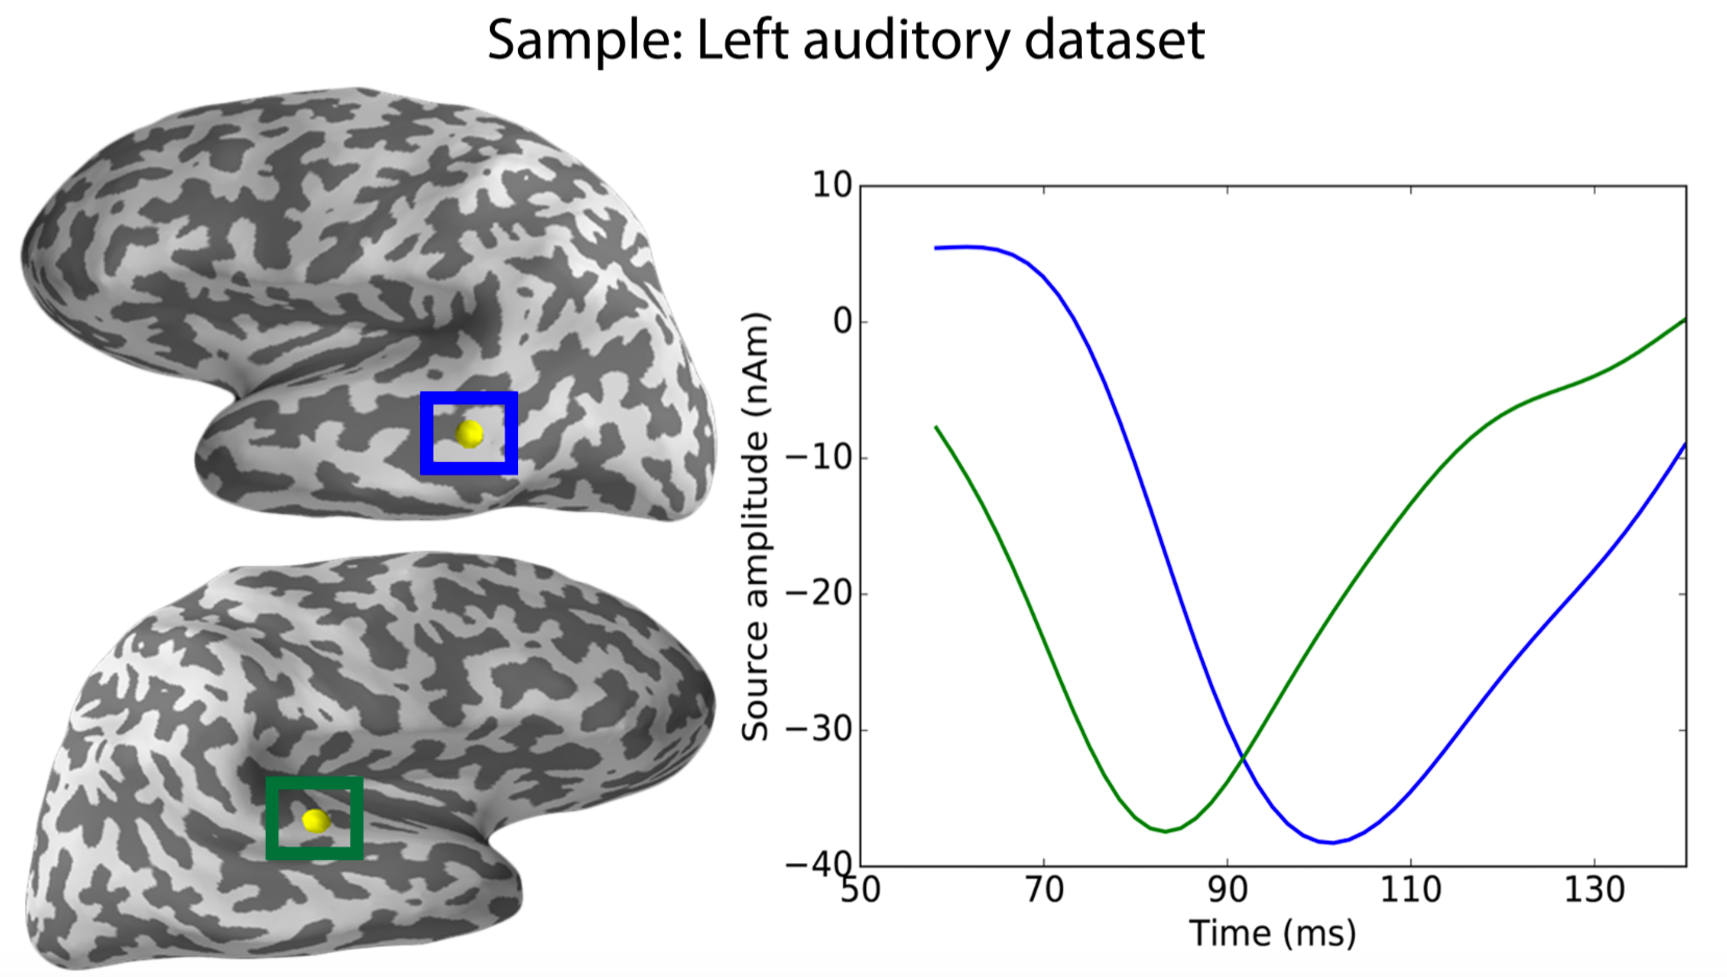
\includegraphics[width=0.95\textwidth]{hyperparam_estim/fig_sample}
    \caption{Source reconstruction on MEG auditory data (sample dataset \cite{mne}). Source amplitude of two sources (blue and green) in the right panel and their corresponding positions in the brain on the left. 
    }
%\end{center}
    \label{fig:sample_data}
\end{figure}
Figure~\ref{fig:sample_data} shows the source amplitudes of the two auditory sources and their positions in the brain when estimating a hyperparameter per source. When using a single hyperparameter on the convex norm $\ell_{2,1}$, multiple spurious sources are found as active which replicates the simulation on Figure~\ref{fig:mxne_vs_irmxne}-(a). These source estimates in Figure~\ref{fig:sample_data} correspond to the M100 peak (peak around 100 ms) generated in the vicinity of the bilateral auditory cortices in superior temporal gyri (the relevant auditory area).


%----------Link between MM & HBM------------------------------------------------------------
\section{Link between MM and special case of HBM}\label{link_hbm_mm}

We start this section by recalling how majorization-minimization works
when addressing variational formulations with concave, hence non-convex, regularization. It is followed by an introduction to hierarchical Bayesian models with Gamma hyper-priors. Then, we explain how these seemingly different approaches can lead to the exact same regression algorithm.
From this, we detail how different Bayesian inference strategies using MCMC
sampling can more precisely explore the landscape of the posterior distribution of the HBM model and provide multiple possible solutions to the sparse regression problem compared to MM.

\subsection{Majorization-Minimization: MM}
\label{section:MM}

Majorization-Minimization (MM) strategies consist in replacing a difficult optimization problem with a series of easier ones that are obtained by upper bounding the objective function, often by a convex majorant.
%
In the context of inverse problems or high-dimensional statistics using sparsity constraints, MM has been successfully applied to address non-convex regularization terms. An example is the regression model with $\ell_{2,p}$-quasi-norms regularization over the groups when $0<p<1$: the desired estimate $\hat{\bfX}$ is defined as one of potentially multiple minimizers of:

\begin{equation} \label{eq:L2pReg}
\hat{\bfX} \in \argmin_{\bfX\in\R^{SO \times T}} \frac{1}{2} \fronormsq{\bfM - \bfG \bfX}  + \lambda \sum_{i=1}^S \fronorm{\bfX{[i]}}^p \enspace,
\end{equation}
similarly to Equation~\eqref{eq_reg} (page~\pageref{eq_reg}), where $\lambda > 0$ is the regularization parameter balancing the data fit and the penalty term, and $\mathbf{X}[i]$ defines the block of source $i$ ($\RR^T$ if $O=1$ or $\RR^{3\times T}$ if $O=3$). One possible MM approach to solve Equation~\eqref{eq:L2pReg} with $p=0.5$ would consist of minimizing a sequence of non-smooth convex surrogate functions where the non-convex regularization (irMXNE solver) is replaced by a weighted $\ell_{2,1}$ norm similar to MxNE solver~\cite{strohmeier-etal:16}. In each iteration, the weights are derived from the current estimate of $\bfX$.

Due to the concavity of the non-decreasing function $\bfX\mapsto\sqrt{\fronorm{\bfX}}$, it is upper bounded by its tangent and a first order Taylor expansion at the current estimate $\bfX{[i]}$ provides an upper bound that can be used to construct the non-smooth convex surrogate problem. By solving this sequence of surrogate problems, the value of the non-convex objective function is guaranteed to decrease. However, due to the non-convexity, only convergence towards a local minimum can be guaranteed.

For the problem in Equation~\eqref{eq:L2pReg} with $p=0.5$, the $k^{th}$ iteration of the MM scheme reads:
\begin{equation}
\label{eq:MM}
\fl \quad \bfX^{(k)} \in \argmin_{\bfX\in\R^{SO \times T}} \frac{1}{2} \fronormsq{\bfM - \bfG \bfX}  + \lambda \sum_{i=1}^S \frac{ \fronorm{\bfX{[i]}} }{ \bfw^{(k-1)}[i]},
\end{equation}
with:
\begin{equation*}
\bfw^{(k-1)}[i] = 2 \sqrt{\fronorm{\bfX^{(k-1)}[i]}} \enspace.
\end{equation*}
As each weight $\bfw^{(k)}[i]$ is a non-decreasing function of $\fronorm{\bfX^{(k)}[i]}$, sources with high amplitudes in one iteration will be less penalized in the next iteration and can better explain the data $\bfM$. Sources for which $\fronorm{\bfX^{(k)}[i]} = 0$ at a certain iteration $k$ are effectively pruned from the model for all following iterations. Using MM therefore leads to a solution that explains the data with fewer active locations $i$ compared to a standard $\ell_{2,1}$ norm regularized solution.\\
Note that a default initialization consists in setting $\bfw^{(0)}[i]=1, \forall i \in [1,\cdots, S]$~\cite{strohmeier-etal:16}.

To exploit existing fast solvers for the $\ell_{2,1}$ regularized problems~\cite{strohmeier-etal:16,Ndiaye_Fercoq_Gramfort_Salmon15}, we reformulate the weighted subproblem and apply the weights by scaling the matrix $\bfG$ with a diagonal matrix $\bfW^{(k)} \in \bbR^{SO \times SO}$ given by:
\begin{eqnarray} \label{eq:weights}
\bfW^{(k)} = \mathrm{diag}(\bfw^{(k)} \otimes \mathbf{1}_{O}) \enspace ,
\end{eqnarray}
where $\bfw^{(k)} \in \bbR^{S}$, $\mathbf{1}_{O}\in\R^O$ is a vector of ones and $\otimes$ is the Kronecker product.
Defining $\tilde{\bfG}^{(k)}=\bfG \bfW^{(k-1)}$, the reformulated problem reads:
\begin{eqnarray}\label{eq:lasso_new_gram}
\tilde{\bfX}^{(k)} \in \argmin_{\bfX\in\R^{SO \times T}} \frac{1}{2}\fronormsq{\bfM - \tilde{\bfG}^{(k)} \bfX}  + \lambda \sum_{i=1}^S \fronorm{\bfX[i]} \enspace .
\end{eqnarray}

The convergence of each weighted $\ell_{2,1}$ (MxNE) is controlled by monitoring the duality gap (see Section~\ref{section:duality_gap}). For more details about convex duality of optimization with sparsity-inducing penalties, refer to~\cite{bach2012optimization}.\\
As mentioned in Section~\ref{section:duality_gap}, the minimum of the primal objective function $f_p(\mathbf{X})$ is bounded below by the maximum of the dual objective function $f_d(\mathbf{Y})$, \textit{i.e.}\\
$f_d(\mathbf{Y}^\star)\leq f_p(\mathbf{X}^\star)$ where $\mathbf{X}^\star$ and $\mathbf{Y}^\star$ are the optimal solutions of the primal and the dual objective functions respectively. If strong duality holds, the duality gap defined as $\eta=f_p(\mathbf{X})-f_d(\mathbf{Y})$ would be zero at the optimum.\\
Due to Slater's conditions~\cite{Boyd_Vandenberghe04}, the strong duality holds for the MxNE subproblem and the gap can be used to check the convergence of Equation~\eqref{eq:MM}. Based on Fenchel-Rockafellar duality theorem~\cite{rockafellar:1997}, one dual objective function associated with the primal objective function:
\begin{equation}
\begin{split}
f_p(\mathbf{X}) & = \frac{1}{2}\|\mathbf{M}-\mathbf{GX}\|_{Fro}^2+\lambda\mathcal{P}(\mathbf{X}) \\
& = \frac{1}{2}\|\mathbf{M}-\mathbf{GX}\|_{Fro}^2+\lambda\sum_{i=1}^S\|\mathbf{X}[i]\|_{Fro}
\end{split}
\end{equation}
is given by:
\begin{equation}
f_d(\mathbf{Y})=-\frac{1}{2}\|\mathbf{Y}\|_{Fro}^2+Tr(\mathbf{Y}^\top\mathbf{M})-\lambda\mathcal{P}^\star(\mathbf{G}^\top\mathbf{Y}/\lambda)
\end{equation}
where $\mathcal{P}^\star$ is the Fenchel conjugate of $\mathcal{P}$, which is the indicator function of the associated dual form. For a full derivation, see~\cite{Gramfort_Kowalski_Hamalainen12}. Moreover, the Karush-Khun-Tucker (KKT) conditions of the Fenchel-Rockafellar duality theorem give a natural mapping from
the primal to the dual space, which is given by a scaling of the residual $\tilde{\mathbf{Y}}=\mathbf{M}-\mathbf{GX}$, as shown in~\cite{Gramfort_Kowalski_Hamalainen12}.\\
In practice, we terminate the optimization scheme for solving MxNE when the estimate at the $k^{th}$ iteration is $\epsilon$-optimal with $\epsilon=10^{-6}$~\cite{strohmeier-etal:16}.\\

{\fontsize{4}{4}\selectfont
%above is to make smaller fonts in algorithm
\begin{algorithm}[t]
\SetKwInOut{Input}{input}
\SetKwInOut{Init}{init}
\SetKwInOut{Parameter}{param}
\caption{\textsc{$\ell_{2,p}$ MM algorithm with $p=0.5$ (Adaptive \ac{lasso}) - iterative reweighted MxNE}}
\Input{$\bfM, \bfG,\lambda > 0, \bfW^{(0)} \geqslant 0,\epsilon > 0, \tau > 0$ and $K$ }
% \Parameter{ To add }
%\Init{$\bfW^{(1)}=I_{dn\times dn}$ }
\For{
        $k = 1$ to $K$
    }
    {
		$\tilde{\bfG}^{(k)} = \bfG \bfW^{(k-1)}$

		Get $\tilde{\bfX}^{(k)}$ by solving Equation~\eqref{eq:lasso_new_gram} at $\epsilon$-precision as done in Algorithm~\ref{alg:mxne_activeset}.

		Update $\hat{\bfX}^{(k)} = \bfW^{(k-1)} \tilde{\bfX}^{(k)}$

	    Update $\bfW^{(k)}=\mathrm{diag}(\bfw^{(k)} \otimes \mathbf{1}_{O})$ where $\bfw^{(k)}[i] = 2 \sqrt{\fronorm{\hat{\bfX}^{(k)}[i]}}$  $\forall i\in [1, \cdots, S]$

		\If{ $\norm{\hat{\bfX}^{(k)}-\hat{\bfX}^{(k-1)}}_{\infty} \leq \tau$}{Break}

     }
%\Return{$\hat{\bfX}^{(k)}$}
\label{alg:adpative_lasso}
\end{algorithm}
}

For solving the weighted MxNE subproblems, the \ac{BCD} scheme was used~\cite{tseng}, which for the problem at hand converges faster than \ac{FISTA} (See Section~\ref{section:comparison_solvers}). The subproblem per block has a closed-form solution, which involves applying the group soft-thresholding operator, the proximity operator associated to the $\ell_{2,1}$-mixed-norm~\cite{gramfort2012mixed,strohmeier-etal:16}.

{\fontsize{4}{4}\selectfont
%above is to make smaller fonts in algorithm
\begin{algorithm}[t]
\SetKwInOut{Input}{input}
\SetKwInOut{Init}{init}
\SetKwInOut{Parameter}{param}
\caption{\textsc{MxNE with BCD and active set strategy}}
\Input{$\bfM, \bfG,\lambda > 0, \epsilon > 0$, and $S$ }
% \Parameter{ To add }
\Init{$\mathbf{X}=0$, $\Gamma=\{\}$, $\eta=f_p(\mathbf{X})-f_d(\mathbf{Y})$}
\For{
        $i = 1$ to $S$
    }
    {
		$\mu[i] = \|\mathbf{G^\top_i\mathbf{G}_i}\|^{-1}$
     }
\While{
		$\eta \geq \epsilon$
	  }
	  {
	  	$\Gamma^\star = \{i \hspace{3pt} | \hspace{3pt} \|\mathbf{G}_i^\top(\mathbf{M}-\mathbf{GX})\|_{Fro} > \lambda\}$

	  	$\Gamma = \Gamma\cup \Gamma^\star$

	  	Define $\mathbf{G}^\Gamma$ and $\mathbf{X}^\Gamma$ by restricting $\mathbf{G}$ and $\mathbf{X}$ to $\Gamma$

	  	$\mathbf{X}^{\star}_\Gamma \leftarrow$ Output of Algorithm~\ref{alg:mxne_bcd} with $\mathbf{\mu}, \mathbf{G}^\Gamma$, and $\mathbf{X}_0=\mathbf{X}_\Gamma$

	  	$\mathbf{X}[\Gamma, :] = \mathbf{X}^{\star}_\Gamma$

	  	$\eta=f_p(\mathbf{X})-f_d(\mathbf{Y})$
	  }
%\Return{$\hat{\bfX}^{(k)}$}
\label{alg:mxne_activeset}
\end{algorithm}
}

{\fontsize{4}{4}\selectfont
%above is to make smaller fonts in algorithm
\begin{algorithm}[t]
\SetKwInOut{Input}{input}
\SetKwInOut{Init}{init}
\SetKwInOut{Parameter}{param}
\caption{\textsc{MxNE with BCD}}
\Input{$\bfM, \bfG,\bfX, \mathbf{\mu}, \lambda > 0, \epsilon > 0$, and $S$ }
% \Parameter{ To add }
\Init{$\eta=f_p(\mathbf{X})-f_d(\mathbf{Y})$}
\While{
		$\eta \geq \epsilon$
	  }
	  {
	  	\For{
	  			$i=1 \in S$
	  		}
	  		{
	  			$\mathbf{X}[i]\leftarrow$ Solve Equation~\eqref{eq_bcd_glasso} with $\mathbf{X}, \mathbf{\mu}$, and $\mathbf{M}$
	  		}
	  	$\eta = f_p(\mathbf{X})-f_d(\mathbf{Y})$
	  }
\label{alg:mxne_bcd}
\end{algorithm}
}

After convergence, we re-apply the scaling to $\tilde{\bfX}$ to obtain $\hat{\bfX}$:
\begin{equation}
    \label{eq:MM_weights}
    \bfX^{\star(k)} = \bfW^{(k-1)} \tilde{\bfX}^{(k)} \enspace .
\end{equation}
The reformulation through Equation~\eqref{eq:lasso_new_gram} and Equation~\eqref{eq:MM_weights} avoids any division by zero when $\bfX^{(k-1)}=0$. The above procedure, which matches the strategy of the Adaptive \ac{lasso} estimator~\cite{Zou06}, is expressed as pseudo-code in Algorithm~\ref{alg:adpative_lasso}.

%%%%%%%%%%%%%%%%%%%%%%%%%%%%%%%%%%%%%%%%%%%%%%%%%%%%%%%%%%%%%%%%%%%%%%%%%%%%%%%
\subsection{Hierarchical Bayesian Modeling}
\label{section:HBM}
%%%%%%%%%%%%%%%%%%%%%%%%%%%%%%%%%%%%%%%%%%%%%%%%%%%%%%%%%%%%%%%%%%%%%%%%%%%%%%%

In this section, we formulate the inference problem defined by Equation~\eqref{eq_linmeeg} (page~\pageref{eq_linmeeg}) and the regularization strategy with $\ell_{2,p}$-quasinorm from a Bayesian perspective~\cite{KaSo05,Lu14}: the Bayesian approach incorporates prior beliefs about the model parameters in terms of probability distributions. Under the Additive, White Gaussian Noise (AWGN) assumption, the likelihood of the model is given by:
\begin{eqnarray} \label{eq:like}
\like &\propto \exp \left( - \frac{1}{2} \fronormsq{\bfM - \bfG \bfX} \right) \enspace.
\end{eqnarray}

From Equation~\eqref{eq:L2pReg} we can construct the $\ell_{2,p}$ group prior as:

\begin{equation} \label{eq:prior}
\prior \propto \exp \left( - \lambda \sum_{i=1}^S \fronorm{\bfX[i]}^p \right)
= \prod_{i=1}^S \exp \left( - \lambda \fronorm{\bfX[i]}^p \right) \enspace,
\end{equation}
which leads to the following posterior probability density using the Bayes rule:

\begin{equation} \label{eq:post}
\post \propto \exp \left( - \frac{1}{2} \fronormsq{\bfM - \bfG \bfX} - \lambda \sum_{i=1}^S \fronorm{\bfX[i]}^p \right) \enspace.
\end{equation}

To extend Equation~\eqref{eq:prior} to a hierarchical prior model~\cite{mackay2003information}, the scalar $\lambda$ has been replaced by a vector of hyperparameters $\mathbf{\gamma} \in \R^{S}_+$ and for any $p \geq 1$ we write the \emph{conditional $\ell_{2,p}$ prior} as:
\begin{equation} \label{eq:condprior}
\fl \hiprior
= \exp \left( - \sum_{i=1}^S \left( \frac{\fronorm{\bfX[i]}^p}{\mathbf{\gamma}[i]} + \frac{O T}{p} \log(\mathbf{\gamma}[i])\right)\right) \enspace,
\end{equation}
where the logarithmic term accounts for the terms of the normalization that depend on $\mathbf{\gamma}$~\cite{Lu14}. A common choice for a hyper-prior on each $\gamma[i]$ is given by a \emph{Gamma distribution}~\cite{mackay2003information,KaSo05,CaHaPuSo09,Lucka-etal:2012} with shape and scale parameters $\alpha$ and $\beta$:
\begin{align} \label{eq:hyper}
\fl \hyper & \propto \prod_{i=1}^S \mathbf{\gamma}[i]^{\alpha - 1} \exp \left(- \frac{\mathbf{\gamma}[i]}{\beta} \right) \\
& = \exp \left( - \sum_{i=1}^S \left( - \frac{\mathbf{\gamma}[i]}{\beta} + (\alpha - 1) \log(\mathbf{\gamma}[i]) \right) \right) \enspace.
\end{align}
Then, the full posterior over both $\bfX$ and $\gamma$ becomes:

\begin{eqnarray}
\label{eq:full-post}
\fl \hipost \propto \nonumber \\
\fl \hspace{3em} \exp \left( - \frac{1}{2} \fronormsq{\bfM - \bfG \bfX} - \sum_{i=1}^S \left( \frac{\fronorm{\bfX[i]}^p}{\mathbf{\gamma}[i]} + \frac{\mathbf{\gamma}[i]}{\beta} - (\alpha - 1 - \frac{OT}{p}) \log(\mathbf{\gamma}[i]) \right) \right)\enspace.
\end{eqnarray}
The question of how to best derive parameter estimates, in particular how to treat the two different types of parameters $\bfX$ and $\mathbf{\gamma}$, distinguishes different HBM-based inference strategies. Variational Bayesian approaches~\cite{mackay2003information,jordan1999introduction,sato2004hierarchical,FrHaDaKiPhTrHeFlMa08,shervashidze2015learning} and Sparse Bayesian Learning~\cite{tipping2001sparse,wipf2004sparse,Wipf-Nagarajan:2009,zhang2011sparse} approaches rely on approximating or marginalizing the full, joint posterior distribution (Equation~\eqref{eq:full-post}). In contrast, fully-Bayesian strategies~\cite{CaHaPuSo09,Lucka-etal:2012} work with it directly. The most popular one is the full maximum-a-posteriori (\emph{full-MAP}) estimate which is defined as:

\begin{eqnarray}
(\xMAP,\gamMAP) & \in \argmax_{(\bfX,\mathbf{\gamma}) \in\R^{SO \times T} \times \R^{n}_+} \left\lbrace \hipost \right\rbrace \enspace.%,\\
\end{eqnarray}
A common strategy  to compute it is to minimize the \emph{negative log posterior} $-\log \hipost$ by alternating  minimization over $\bfX$ and $\mathbf{\gamma}$ (\emph{block coordinate descent} in optimization):

\begin{equation}\label{eq:AO-X}
\fl \qquad  \bfX^{(k)} \in \argmin_{\bfX\in\R^{SO \times T}} \left\lbrace \frac{1}{2} \fronormsq{\bfM - \bfG \bfX} + \sum_{i=1}^S  \frac{\fronorm{\bfX[i]}^p}{\mathbf{\gamma}^{(k-1)}[i]} \right\rbrace \enspace,
\end{equation}
\begin{equation}\label{eq:AO-gamma}
\begin{split}
\fl \qquad \mathbf{\gamma}^{(k)}[i] \in \argmin_{\mathbf{\gamma}[i]\in \R_+} & \left\lbrace\frac{\fronorm{\bfX^{(k)}[i]}^p }{\mathbf{\gamma}[i]} + \frac{\mathbf{\gamma}[i]}{\beta} - (\alpha - 1 - \frac{OT}{p}) \log(\mathbf{\gamma}[i]) \right\rbrace, \\
& \forall i\in [1,\cdots, S] \enspace. 
\end{split}
\end{equation}
Other fully-Bayesian estimates are defined as integrals of functions of $\bfX$ and $\mathbf{\gamma}$ with respect to the posterior distribution, \textit{e.g.} first or second moment estimates. To compute these high dimensional integrals efficiently, only \ac{MCMC} methods that draw correlated samples from the posterior distribution can be used~\cite{RoCa05,KaSo05}. A commonly used MCMC scheme for HBM is given by \emph{blocked Gibbs sampling}, which alternates as:
\begin{eqnarray}
\bfX^{(k)} &\sim \: p_{post}(\bfX,\mathbf{\gamma}^{(k-1)}|\bfM) &\propto p_{post}(\bfX|\bfM,\mathbf{\gamma}^{(k-1)}) \enspace, \label{eq:AS-X}\\
\mathbf{\gamma}^{(k)} &\sim \: p_{post}(\bfX^{(k)},\mathbf{\gamma}|\bfM) &\propto p_{post}(\mathbf{\gamma}|\bfM,\bfX^{(k)})\enspace. \label{eq:AS-gamma}
\end{eqnarray}
Depending on the purpose of the study, here the main interest is not sampling the posterior distribution for computing the integral-based estimators, but we rather want to explore the different modes of this multi-modal distribution, each of which corresponds to parameters that are both sparse and likely to explain the data.\\
One can notice similar structures in Equations~\eqref{eq:AO-X}-\eqref{eq:AO-gamma} and Equations~\eqref{eq:AS-X}-\eqref{eq:AS-gamma}: in each step, we make use of the conditional structure of the posterior: for $\mathbf{\gamma}$ fixed, we have to solve one $SOT$-dimensional $\ell_{2,p}$ optimization/sampling problems, while for $\bfX$ fixed, we have to solve $S$ 1-dimensional optimization/sampling problems. These two steps will be described in more detail in the sections~\ref{section:hbm_optim} and~ \ref{section:hbm_sampling}.

%----------------HBM Optim------------------------------------------------------------------
\section{HBM optimization in the Bayesian formulation}
\label{section:hbm_optim}
%%%%%%%%%%%%%%%%%%%%%%%%%%%%%%%%%%%%%%%%%%%%%%%%%%%%%%%%%%%%%%%%%%%%%%%%%%%%%%%

The optimization problem defined in Equation~\eqref{eq:AO-X} reduces to an $\ell_{2,p}$-norm regularized regression problem that can be solved as described in Section~\ref{section:MM}. For solving Equation~\eqref{eq:AO-gamma}, we compute the first order optimality condition for each $i$:
\begin{eqnarray}
\label{eq:OptiGamma}
\qquad - \frac{\fronorm{\bfX^{(k)}[i]}^p}{\mathbf{\gamma}[i]^2} + \frac{1}{\beta} - \frac{( \alpha - 1 - \frac{OT}{p})}{\mathbf{\gamma}[i]} &= 0 \enspace,\label{eq:OptiGammaFirst}% \\
\end{eqnarray}

For $\alpha \geqslant O T/p + 1$, the problem in Equation~\eqref{eq:AO-gamma} is convex, and the positive root of Equation~\eqref{eq:OptiGammaFirst} is given by:

\begin{equation}
\mathbf{\gamma}[i] = \beta \left( \nu + \sqrt{ \nu^2 + \frac{\fronorm{\bfX^{(k)}[i]}^p}{\beta}} \right), \qquad \nu \mydef \frac{\alpha - 1 - OT/p}{2} \enspace.
\end{equation}

Note that similar rules to update the noise level were considered in the Bayesian \ac{lasso}~\cite{Park_Casella08,Kyung_Gill_Ghosh_Casella10} and the Scaled \ac{lasso} (see for instance~\cite{Stadler_Buhlmann_vandeGeer10,Dalalyan12}). A difference though is that the update we perform here is on the penalty term, whereas in the mentioned references, it was rather performed on the data-fitting term.

If we furthermore choose $\alpha = O T/p + 1$, then $\nu = 0$ and most terms disappear; Equation~\eqref{eq:AO-X} and~\eqref{eq:AO-gamma} hence read:
\begin{eqnarray}
\bfX^{(k)} &= \argmin_{\bfX\in\R^{SO \times T}} \left\lbrace \frac{1}{2} \fronormsq{\bfM -\bfG \bfX} + \sum_{i=1}^S \frac{\fronorm{\bfX[i]}^p}{\mathbf{\gamma}^{(k-1)}[i]} \right\rbrace \enspace, \label{eq:AO-nu0-X}\\
\mathbf{\gamma}^{(k)}[i] &= \sqrt{\beta} \sqrt{\fronorm{\bfX^{(k)}[i]}^p} \, , \quad \forall i=1,\ldots,S \enspace, \label{eq:AO-nu0-gamma}
\end{eqnarray}
which can be combined into the fixed point iteration:

\begin{equation} \label{eq:AO-nu0-2}
\bfX^{(k)} = \argmin_{\bfX\in\RR^{SO \times T}} \left\lbrace \frac{1}{2} \fronormsq{\bfM -\bfG \bfX} + \frac{2}{\sqrt{\beta}} \sum_{i=1}^S  \frac{\fronorm{\bfX[i]}^p}{2 \sqrt{\fronorm{\bfX^{(k-1)}[i]}^p}} \right\rbrace \enspace .
\end{equation}
If we compare Equation~\eqref{eq:AO-nu0-2} with Equation~\eqref{eq:MM}, we see that we re-derived the MM algorithm for $p=1$ as an alternating optimization scheme to compute the \emph{full-MAP} estimate for a specific HBM, namely using a conditional $\ell_{2,1}$ group prior and a Gamma hyper-prior with $\alpha = OT + 1$ and $\beta = 4/\lambda^2$. Using $\bfw^{(0)}[i] := 1$ in the MM scheme corresponds to starting with $\mathbf{\gamma}[i]^{(0)} := 1/\lambda =  2/\sqrt{\beta}$.\\

From previous work~\cite{strohmeier-etal:16} we know that due to the non-convexity, a good initialization of the weights $\bfw^{(0)}[i]$ in the MM algorithm is crucial for its performance, but aside uniform initialization, only heuristic initialization strategies were used, \textit{e.g.} using the same re-weighting as in the sLORETA method~\cite{Pa02}. In this thesis, we leverage the re-interpretation of the MM algorithm through the HBM framework to obtain multiple initializations in a systematic fashion, namely as samples drawn from the full posterior. In this way, we can not only reach better local minima, but more importantly, we can identify and characterize multiple possible sparse solutions. Such plausible solutions to the sparse regression problem in Equation~\eqref{eq_linmeeg} are the modes of the posterior distribution (Equation~\eqref{eq:full-post}) with different relative probability masses.

%----------------Sampling-------------------------------------------------------------------
\section{Posterior Sampling}
\label{section:hbm_sampling}
%%%%%%%%%%%%%%%%%%%%%%%%%%%%%%%%%%%%%%%%%%%%%%%%%%%%%%%%%%%%%%%%%%%%%%%%%%%%%%%

As outlined in Equations~\eqref{eq:AS-X} and~\eqref{eq:AS-gamma} in Section~\ref{section:HBM}, we sample the full posterior $\hipost$ by blocked Gibbs sampling, \ie we alternate between sampling the conditional distributions $p_{post}(\bfX|\bfM,\mathbf{\gamma}^{(k-1)})$ and $p_{post}(\mathbf{\gamma}|\bfM,\bfX^{(k)})$. The conditional $p_{post}(\bfX|\bfM,\mathbf{\gamma}^{(k-1)})$ is a high dimensional distribution composed of a Gaussian likelihood and an $\ell_{2,p}$ prior, where our main interest here is $p = 1$. It was demonstrated in~\cite{Lu12} that \termabb{single component Gibbs sampling}{SC Gibbs} is an efficient MCMC technique to sample such distributions. For the specific $\ell_{2,p}$ priors used here, \emph{slice sampling} can be used to perform the sub-steps in SC Gibbs sampling, namely the sampling of the one-dimensional single-component conditional densities. The resulting \emph{Slice-Within-Gibbs} sampler was examined in~\cite{Lu16}. For completeness, the details of the implementation are given in Section~\ref{sec:DetailsGammaSampler}.

Following Equation~\eqref{eq:full-post}, the conditional $p_{post}(\mathbf{\gamma}|\bfM,\bfX^{(k)})$ factorizes over groups $i$:
\begin{equation}
\fl \qquad p_{post}(\mathbf{\gamma}[i]|\bfM,\bfX^{(k)}) \propto \exp \left( -\frac{\fronorm{\bfX^{(k)}[i]}^p}{\mathbf{\gamma}[i]} - \frac{\mathbf{\gamma}[i]}{\beta} + (\alpha - 1 - O T/p) \log(\mathbf{\gamma}[i]) \right) \enspace. \label{eq:conPostGammai}
\end{equation}
For the case of $\alpha = O T/p + 1$, which is our main interest due to its connection to MM revealed in the previous section, Equation~\eqref{eq:conPostGammai} reduces to:
\begin{equation}
\fl \qquad p_{post}(\mathbf{\gamma}[i] |\bfM, \bfX^{(k)}) \propto \exp \left(- \frac{\fronorm{\bfX^{(k)}[i]}^p}{\mathbf{\gamma}[i]} \right) \exp \left(- \frac{\mathbf{\gamma}[i]}{\beta} \right) \enspace, \label{eq:conPostGammaiRed}
\end{equation}
which can be sampled with a simple accept-reject algorithm as described in Section~\ref{sec:DetailsGammaSampler}. The complete procedure is described in Algorithm~\ref{alg:sampling}. Therein, $K_0$ refers to the burn-in size, \textit{i.e.} the initial samples that are discarded, $K$ to the sample size of the blocked Gibbs sampler and $K_{SC}, K_{SS}$ to the sample sizes of the SC Gibbs and the slice sampler that carries out the sampling in the sub-steps.

{\fontsize{4}{4}\selectfont
%above is to make smaller fonts in algorithm
\begin{algorithm}[t]
\SetKwInOut{Input}{input}
\SetKwInOut{Init}{init}
\SetKwInOut{Parameter}{param}
\caption{\textsc{Block Gibbs Sampling scheme}}
\Input{$\bfM, \bfG $, $\bfX^{(-K_0)}$, $\mathbf{\gamma}^{(-K_0)}$, $K_0$, $K$, $K_{SC}$, $K_{SS}$, $\alpha$, $\beta$}
% \Parameter{}

\For{
        $k = -K_0+1$ \textbf{to} $K$
    }
    {%Sample $(\bfX,\gamma) \sim p_{post}(\bfX,\gamma |\bfM)$ via \textbf{Block Gibbs:}
    Set $\bfX^{(k)} = \bfX^{(k-1)}$.\\
    \For{
    		$k_{SC} = 1$ \textbf{to} $K_{SC}$
    		}
    		{
    		Draw a random permutation $P$ of $\{1,\ldots,S\}$\\
    		\For{
    			$l \in P$
    			}
    			{
			Sample $\bfX^{(k)}[i,j] \sim p_{post}(\bfX[i,j]|\bfX^{(k-1)}[-(i,j)],\bfM,\mathbf{\gamma}^{(k)})$, $\forall (i,j)\in [l]$ - via $K_{SS}$ steps of \textbf{Slice Sampling} Algorithm~\ref{alg:Slice}.
			}
		}
	{Sample $\gamma^{(k)}_{i} \sim p_{post}(\gamma_{i}|\bfM,\bfX^{(k)})$, $\forall i =1,\ldots,n$ via \textbf{Accept-Reject} Algorithm~\ref{alg:acceptreject}.}

    }
\Return{$\{\bfX^{(k)},\mathbf{\gamma}^{(k)}\}_{k=1}^K$}
\label{alg:sampling}
\end{algorithm}
}


\subsection{Slice-Within-Gibbs Sampler for Parameter Update}\label{sec:DetailsGammaSampler}

Within the Algorithm \ref{alg:sampling}, to update a group $\bfX[l]$, we need to sample from all the one-dimensional SC densities:
\begin{equation}
p_{post}(\bfX[i,j]|\bfX^{(k-1)}[-(i,j)],\bfM,\mathbf{\gamma}^{(k)}), \qquad (i,j) \in [l] \enspace ,
\end{equation}
where $\bfX[-(i,j)]$ refers to all the coefficients of matrix $\bfX$ except the term $(i,j)$.

In order to implement this efficiently, we can precompute several terms and make use of the specific spatio-temporal group structure of the posterior. We first derive the part of the likelihood as in Equation \eqref{eq:like} that depends on a given index pair $(i,j) \in [l]$:
\begin{gather*}
\fl \hspace{2cm} \frac{1}{2} \fronormsq{\bfM - \bfG \bfX} = \sum_{j'}^{T} \frac{1}{2} \norm{\bfM[:,j'] - \bfG \bfX[:,j']}_2^2 \\
\proptoab{j} \\
\fl \hspace{3cm} \frac{1}{2} \norm{\bfM[:,j] - \bfG \bfX[:,j]}_2^2 = \frac{1}{2} \norm{\bfM[:,j] - \left( \bfG[:, -i] \bfX[-i,j] + \bfG[:, i] \bfX[i,j] \right)}_2^2 \\
\proptoab{i} \\
\fl \hspace{2cm} \frac{1}{2} \norm{\bfG[:,i]}_2^2 \, \bfX[i,j]^2 + \bfG[:,i]^\top \left(\bfM[:,j] - \bfG[:,-i] \bfX[-i,j] \right) \, \bfX[i,j] \\
\fl \hspace{-6.5cm} = \frac{1}{2} \norm{\bfG[:,i]}_2^2 \, \bfX[i,j]^2 \\
\fl \hspace{5cm} + \left( \left( \bfG^\top \bfM\right)[i,j] - \left({\bfG[:,i]}^\top \bfG\right) \bfX[:,j] - \norm{\bfG[:,i]}_2^2 \right) \, \bfX[i,j]\\
\fl\hspace{3cm} := a z^2 + b z \enspace , \quad \text{with} \quad z := \bfX[i,j] \enspace , \quad a := \frac{1}{2} \norm{\bfG[:,i]}_2^2 \enspace , \\
\fl \hspace{1.5cm} b :=  \left( \bfG^\top \bfM\right)[i,j] - \left({\bfG[:,i]}^\top \bfG\right) \bfX[:,j] - \norm{\bfG[:,i]}_2^2
\end{gather*}
where $\proptoab{j}$ means propotional for each $j$, and $:=$ assign the equation to a specific reformulation.

Note that $\norm{\bfG[:,i]}_2^2 $ and $\bfG^\top \bfM$ can be precomputed. The challenging part in the computation of $b$ is to compute ${\bfG[:,i]}^\top \bfG$, as one typically does not want to pre-compute the $SO \times SO$ matrix $\bfG^\top \bfG$ and hold it in memory. However, to update all the $TO$ components of the $l^{th}$ group (\textit{e.g.} in the visual evoked fields example, $T = 211$, $O = 3$) one only needs the $O \times SO$ matrix ${\bfG[:,[l]]}^\top \bfG$. Thus, we compute ${\bfG[:,[l]]}^\top \bfG$ at the start of updating group $\bfX[l]$ and hold it in memory throughout the bloc update. Besides this, the most costly operation to compute $b$ is a dot product of vectors of size $SO$. Next, we derive the part of the prior \eqref{eq:condprior} that depends on $\bfX[i,j], (i,j) \in [l]$:
\begin{gather*}
\fl \hspace{-5cm} \sum_{l=1}^S \left( \frac{\fronorm{\bfX[l]}^p}{\mathbf{\gamma}{l}} + \frac{O T}{p} \log(\mathbf{\gamma}[l])\right) \quad \\
\fl \hspace{2cm} \proptoab{\bfX[i,j], (i,j) \in [l]} \quad \mathbf{\gamma}[l]^{-1} \fronorm{\bfX[l]}^p =  \mathbf{\gamma}[l]^{-1} \left( \sum_{(i',j') \in [l]} \bfX[i',j']^2  \right)^{p/2}  \nonumber \\
\fl \hspace{9.3cm} = \mathbf{\gamma}[l]^{-1} \left(\bfX[i,j]^2 + \sum_{(i',j') \in [l] \atop (i',j') \neq (i,j)} \bfX[i',j']^2  \right)^{p/2} \\
\fl \hspace{5cm} := c \left(z^2 + d \right)^{p/2} \enspace ,
\end{gather*}
with $c$ and $d$ defined and computed in an obvious way. Taken together, to update $\bfX[i,j]$, we have to sample from the one-dimensional density:
\begin{equation}
p(z) \propto \exp \left(- a z^2 - b z \right) \exp \left(- c \left(z^2 + d \right)^{p/2} \right) =: p_1(z) p_2(z) \enspace . \label{eq:SCdensity}
\end{equation}
We take advantage of the fact that \eqref{eq:SCdensity} factorizes in a Gaussian likelihood part $p_1(z)$ and a symmetric, log-concave prior part $p_2(z)$, and use a generalized form of slice sampling \cite{Ne03,RoCa05} as described in more detail in \cite{Lu16} and summarized in Algorithm \ref{alg:Slice}. Determining $S_2^y$ in our case is trivial:
\begin{align}
\fl p_2(z) \geqslant y \quad & \Leftrightarrow \quad c \left(z^2 + d \right)^{p/2} \leqslant - \log(y) \quad \\
\fl & \Leftrightarrow |x| \leqslant \left( \left( \frac{- \log(y)}{c} \right)^{2/p} - d \right)^{1/2}
\end{align}
Then, we use a slightly modified, more robust version of the fast table-based algorithm described in \cite{Ch12} to sample from the truncated Gaussian distribution $p_1(z) \mathbf{\mathbbm{1}}_{S^y_2}(z)$. As initialization for $z$, we always choose the current value of $\bfX[i,j]$.

{\fontsize{4}{4}\selectfont
%above is to make smaller fonts in algorithm
\begin{algorithm}[t]
\SetKwInOut{Input}{input}
\SetKwInOut{Init}{init}
\SetKwInOut{Parameter}{param}
\caption{\textsc{Slice Sampling}}
\Input{$p(z) \propto p_1(z) p_2(z), z, K_{(SS)} $}
\For{
     $k = 1$ to $K_{SS}$
    }
    {
    Draw $y$ uniformly from $\left[0,p_2(z)\right]$ (vertical move).\\
    Determine $S_2^y \mydef \left\lbrace z \;|\; p_2(z) \geqslant y \right\rbrace$\\
	Draw $z$ from $p_1(z) \mathbf{\mathbbm{1}}_{S^y_2}(z)$ (weighted horizontal move).
    }
{\Return{$z$} as a sample of $p(z)$}
\label{alg:Slice}
\end{algorithm}
}


\subsection{Accept-Reject Sampler for Hyperparameter Update} \label{sec:DetailsGammaSampler}

The conditional density \eqref{eq:conPostGammaiRed} is of the type
\begin{equation}
\fl \qquad p(x) \propto \exp \left(- \frac{c}{x} \right) \exp \left(- \frac{x}{\beta} \right) \enspace, \qquad c, \beta \geqslant 0.
\end{equation}
Note that the first factor is monotonically increasing with limit $0$ for $x \searrow 0$ and limit $1$ for $x \rightarrow \infty$, while the second factor is proportional to a simple exponential distribution (\lcf Figure \ref{fig:AccRejSketch}). We can therefore easily construct a dominating density $g(x) \geqslant p(x)$ to carry out accept-reject sampling \cite[Section 2.3.2]{RoCa05} to generate a sample $z \sim p$: we generate $y \sim g$, $u \sim \mathcal{U}_{[0,1]}$ and accept $z = y$ if $u \leqslant p(y)/g(y)$ and repeat otherwise. Choosing $g(x) = \exp \left(- x/\beta\right)$ would yield a valid sampling density but this choice becomes inefficient with increasing $c$. Therefore, we split the sampling density into two parts:
\begin{equation}
g(x) = 
\begin{cases}
\hat p & \text{if} \hspace{10pt} x < \tilde{x} \\
\exp \left(- \frac{x}{\beta} \right)	& \text{otherwise}  \enspace,
\end{cases}
\label{eq:ARsamplingDensity}
\end{equation}
where $\hat p = \max_x p(x)$ is the maximal probability attained at $\hat x = \argmax_x p(x) = \sqrt{\beta c}$ and $\tilde{x} = \beta c/\hat x + \hat x$ is the solution to $\exp \left(- x/\beta\right) = \hat p$ (\textit{cf.} Figure~\ref{fig:AccRejSketch}). Sampling from~\eqref{eq:ARsamplingDensity} is then straightforward using $v, w \sim \mathcal{U}_{[0,1]}$: if one computes
\begin{equation}
\fl G_{x\geqslant \tilde{x}} = \int_{\tilde{x}}^\infty g(x) \, dx = \beta \exp(- \tilde{x}/\beta), \qquad
G_{x < \tilde{x}} = \int_0^{\tilde{x}} g(x) \, dx = \hat{p} \tilde{x} \enspace,
\end{equation}
then $v <  G_{x\geqslant \tilde{x}} / (G_{x\geqslant \tilde{x}} + G_{x < \tilde{x}})$ determines that we are in the tail, $x > \tilde{x}$, where we can use a simple inverse cumulative distribution method to draw a proposal from $g(x)$ using $w$. If $v$ determines $x \leqslant \tilde{x}$, then $x = w \tilde{x}$ is the proposal. For numerical precision, we only compute logarithms of probabilities and use that for $a > 0$, b$\geqslant 0$:
 \begin{equation}
 \log \left(a +b \right) = \log a + \log \left(1 + \exp \left(b - a \right)\right) \enspace .
 \end{equation}
 The whole sampling scheme is shown in Algorithm~\ref{alg:acceptreject}. We found the scheme to be efficient enough for all of our computations, \textit{i.e.} the chosen $g(x)$ is close enough to $p(x)$ to result in an accepted sample after a few trials. If this had to become a problem, it would be easy to adaptively improve the dominating density.

{\fontsize{4}{4}\selectfont
%above is to make smaller fonts in algorithm
\begin{algorithm}[t]
\SetKwInOut{Input}{input}
\SetKwInOut{Init}{init}
\SetKwInOut{Parameter}{param}
\caption{\textsc{Accept-Reject Algorithm for Hyperparameter Update}}
\Input{$c \geqslant 0, \beta > 0$}
%\Init{$\bfX^{(1)}=\mathbf{0}^{n\cdot d\cdot t}$, $\gamma= \lambda^{-1} \mathbf{1}^{n}$}
% \Parameter{}
Set $\hat x = \sqrt{\beta c}$.\\
Set $\log \hat p = -c/\hat x - \hat x/\beta$.\\
Set $\tilde{x} = \beta c/\hat x + \hat x$.\\
Set $\log G_{x\geqslant \tilde{x}} = \log \beta - \tilde{x}/\beta$.\\
Set $\log G_{x < \tilde{x}} = \log \hat p + \log \tilde{x}$. \\
Set $\log G_{tot} = \log G_{x\geqslant \tilde{x}} + \log\left(1 + \exp\left(G_{x < \tilde{x}} - G_{x\geqslant \tilde{x}}  \right)\right)$.\\
\While{true}
    {
    Draw $u, v, w$ uniformly from $\left(0,1\right)$.\\
    \If{$\log v + \log G_{tot} < \log G_{x\geqslant \tilde{x}}$}{
		Set $W = \log w - \tilde{x}/\beta$.\\
		Propose $x = - \beta W$:\\
		\If{$\beta \log(u) < c/W$}{\Return{$x$} (acceptance)}
    }
    \Else{Propose $x = w \tilde{x}$:\\
    		\If{$\log u + \log \hat{p} < -c/x - x/\beta$}{\Return{$x$} (acceptance)}
    		}
    }
\label{alg:acceptreject}
\end{algorithm}
}

\begin{figure}[tb]
   \centering
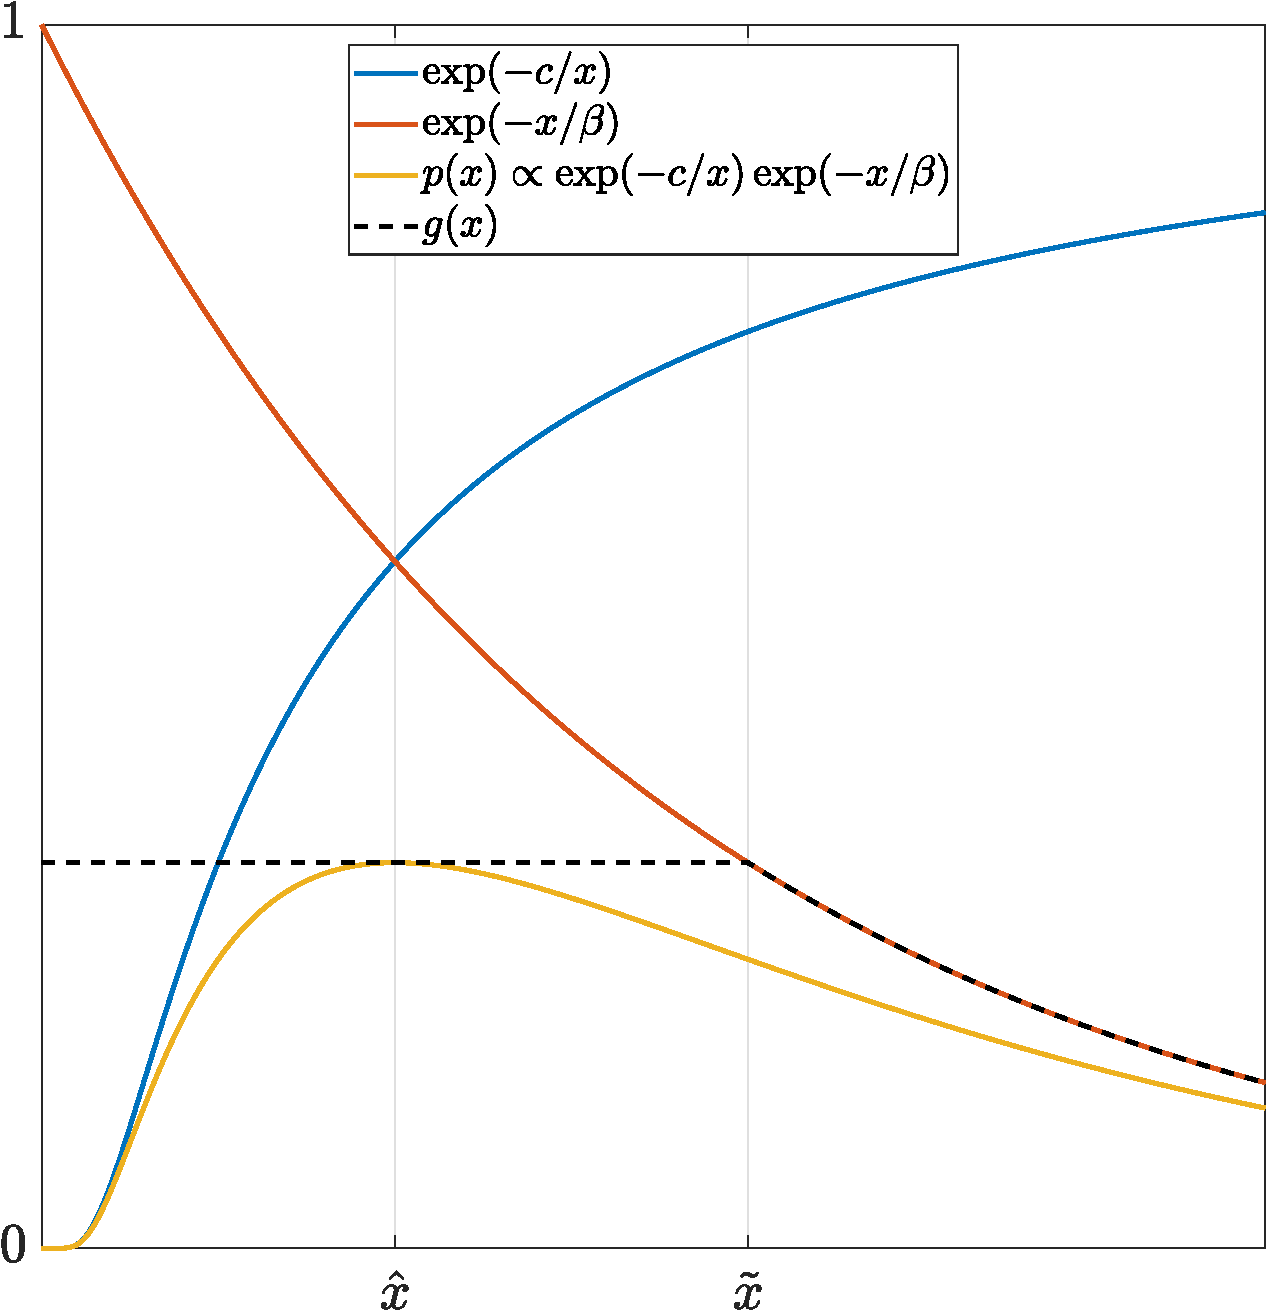
\includegraphics[width = 0.4\textwidth]{hbm/AcceptRejectSketch}
\caption{Sketch of the quantities used in the accept-reject sampling Algorithm~\ref{alg:acceptreject}.}
   \label{fig:AccRejSketch}
\end{figure}


%----------------uncertainty maps-----------------------------------------------------------
%\section{Study of the different modes defining uncertainty maps of inverse problems}

%----------------Experiments-----------------------------------------------------------
\section{Experiments}

\subsection{Study of the different modes defining uncertainty maps of the MEG/EEG inverse problem}

We now examine the benefits of our re-interpretation of the MM algorithm described in Section~\ref{section:MM} as a specific way to compute a full-MAP estimate for a specific HBM as described in Sections~\ref{section:HBM} and ~\ref{section:MM}.
In particular, we investigate how using MCMC sampling of the posterior distribution as described in Section~\ref{section:hbm_sampling} can help getting better initializations for the optimization algorithm.
We first present results for a simulated MEG dataset and then for two experimental MEG/EEG datasets.

\subsubsection{Simulation study}
We generated a realistic simulation based on a free-orientation ($d=3$) source model with $n=7498$ cortical locations and $m=306$ MEG sensors. Two of these locations were selected to be active, one in each hemisphere. One of the sources had a deep ventral location in the inferior occipital gyrus (Figure~\ref{fig:simulated_data}-c), and the second one had a more superficial location in the motor cortex (Figure~\ref{fig:simulated_data}-a). Their corresponding waveforms are shown in Figure~\ref{fig:simulated_data}-b. When passed to the solvers, they are cropped between 40 to 180 ms to keep only the two peaks. This leads to $t=43$ time samples.

\begin{figure}[htp]
	\centering
	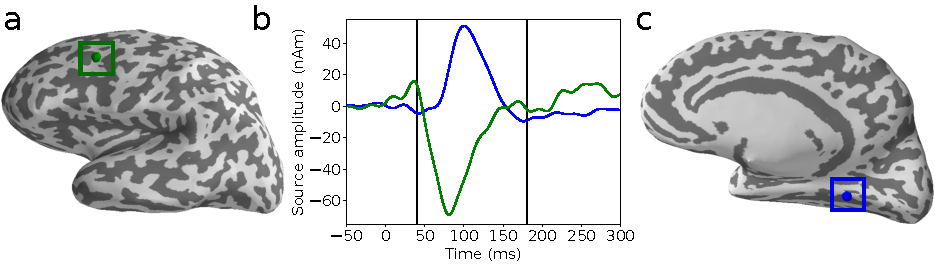
\includegraphics[clip,width=.9\columnwidth]{hbm/simulated_data}%

	\caption{Simulated MEG dataset. a) and c) show superficial and deep sources (hidden in the medial view) locations, respectively. b) gives their corresponding waveforms color-coded by location.}
	\label{fig:simulated_data}
\end{figure}

The aim of the simulation is to answer two separate questions. First, we want to know whether we are able to find better source estimates using MCMC-derived initializations than with the uniformly initialized MM Algorithm~\ref{alg:adpative_lasso}.
For this, we first run the MM Algorithm~\ref{alg:adpative_lasso} using a uniform initialization, \ie $\bfw^{(0)}_{i} = 1, \forall i=1\in [1,\cdots,S]$, with $\lambda = 0.05\lambda_{max}$ where $\lambda_{max}= \max_{1 \leq i \leq S} \fronormsq{(G^\top M)[i]}$ is the smallest regularization value for which no source is found as active using an $\ell_{2,1}$ regularization~\cite{Ndiaye_Fercoq_Gramfort_Salmon15,strohmeier-etal:16}. As described above, this corresponds to computing a full-MAP estimate for the HBM with $p=1$, $\alpha = OT +1 $, $\beta = 4/\lambda^2$ using the alternation scheme \label{eq:AO-nu0-X} initialized with $\mathbf{\gamma}^{(0)}[i] = 1/\lambda, \forall i=1\in [1, \cdots, S]$.

Then, we sampled the corresponding posterior distribution given in Equation~\eqref{eq:full-post} using Algorithm~\ref{alg:sampling} with $K_0 = 300$, $K = 900$, $K_{SC} = K_{SS} = 1$. From each $\mathbf{\gamma}^{(k)}$ of the $K = 900$ obtained $\mathbf{\gamma}$ samples, we construct an initialization $\bfW^{(0)}$ for the MM Algorithm~\ref{alg:adpative_lasso} by setting $\bfw^{(0)}[i] = \lambda \mathbf{\gamma}^{(k)}[i], \forall i=[1,\dots,S]$. Figure~\ref{fig:simu_MM_best_MCMC}-c shows the histogram of the objective function values (computed with Equation~\eqref{eq:lasso_new_gram}) obtained in this way. The vertical black bar shows the value of the objective function of the uniformly initialized MM solver and we can see that some initializations indeed lead to source estimates with a lower objective value. Figure~\ref{fig:simu_MM_best_MCMC}-a and Figure~\ref{fig:simu_MM_best_MCMC}-b show the locations of the estimated sources resulting from uniform and best MCMC-based initialization. For the artificial source in Fig.~\ref{fig:simu_MM_best_MCMC}-a, both results find the exact location, so they are superimposed. For the deeper source in Figure~\ref{fig:simu_MM_best_MCMC}-b, neither result finds the exact position, but the MCMC-based initialization is closer. This means that the result did not only improve from an optimization point of view, but also judged by the quality criteria of the given application.

\begin{figure}[htp]
	\centering
	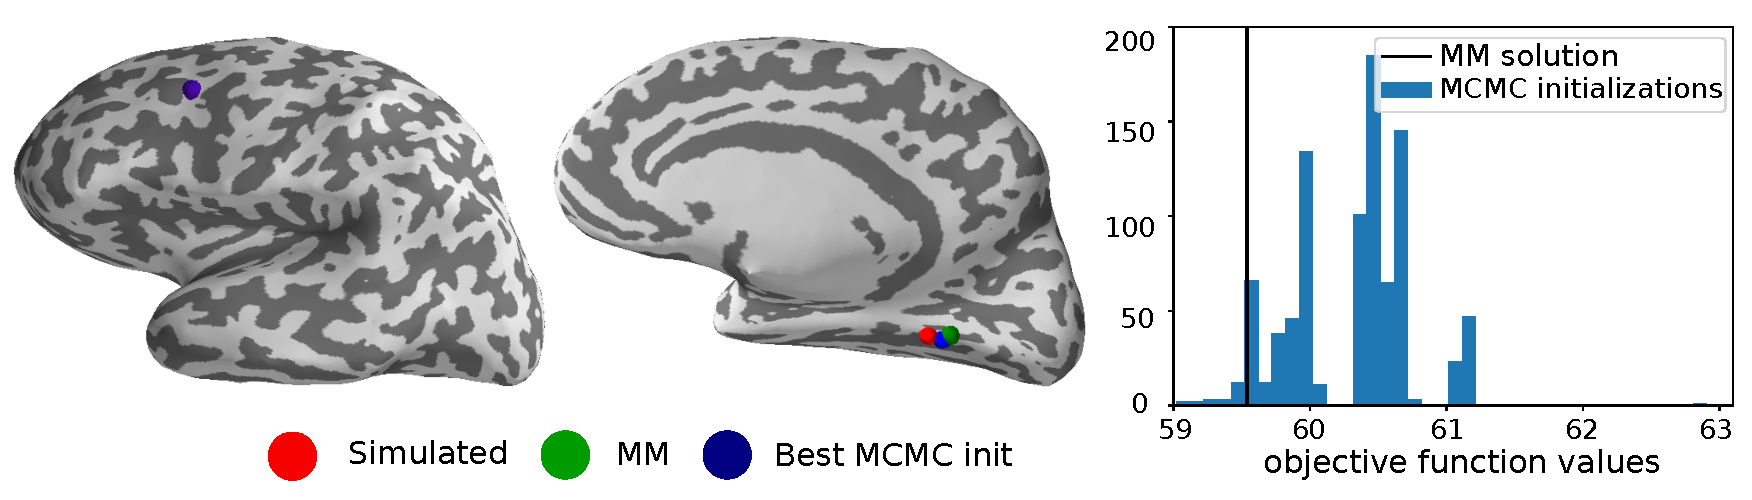
\includegraphics[width=\columnwidth]{hbm/simulated_data_hist_vertices}
	\caption{Location of simulated and estimated sources using the uniformly initialized MM solver (denoted as ``MM'') and best MCMC-based initialization in terms of objective function value. Left: estimation of the artificial source on the left hemisphere. Middle: estimation of the deep source on the right hemisphere. Right: histogram of the objective function value for 900 MCMC initializations. The uniform initialization used for the MM (black vertical line) is not very bad, meaning that the basic MM is able to recover a good source estimate for some configurations. See Figure~\ref{fig:hist_real_datasets} for a case where the basic MM fails.}
	\label{fig:simu_MM_best_MCMC}
\end{figure}

Finding the correct support in a sparse under-determined regression problem like Equation~\eqref{eq_linmeeg} is inherently of combinatorial complexity. In our two approaches, this is reflected in the non-convexity of the objective function (Equation~\eqref{eq:L2pReg}) and the multi-modality of the joint posterior distribution (Equation~\eqref{eq:full-post}), respectively. The second question we want to investigate is whether the methods we developed here can reveal or quantify some of the ambiguity and uncertainty of this sparse support identification problem. Traditional uncertainty quantification (UQ) measures such as variance estimates of $\bfX$ or $\mathbf{\gamma}$ fail to do so as they cannot capture the multi-modality of the posterior in a satisfactory way. In addition, no sample $\bfX^{(k)}$ is exactly sparse: as the posterior distribution is a continuous probability density, the probability of the event $\{\bfX^{(k)}[i] = 0\}$ is zero, which means that the whole support of $\bfX^{(k)}$ is active with probability $1$. Even a thresholded average of the support of $\bfX^{(k)}$ will only reveal the average probability of a location being part of the support. In source analysis, it is arguably more interesting to estimate which networks of sources from different brain areas have most likely produced a given data set, a question left open by these measures. Here, we propose to tackle this question in a different way.

\begin{figure}[htp]
	\centering
	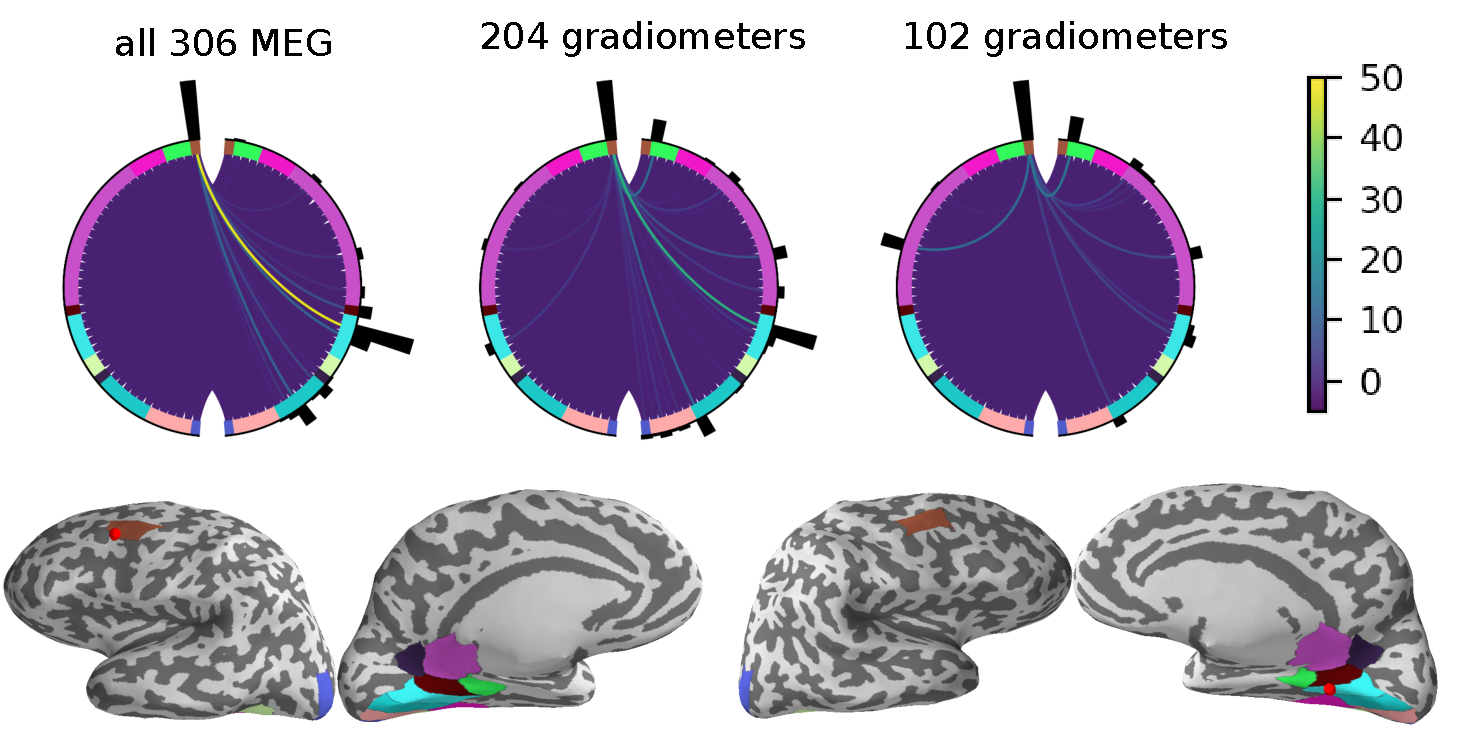
\includegraphics[clip,width=0.98\columnwidth]
{hbm/simulated_circular_plots_new}

	\caption{Source network analysis for simulated data: for a clearer presentation, the set of 900 initializations was thinned to the 100 that gave the lowest objective function (Equation~\eqref{eq:L2pReg}). The first row of sub-figures displays the support of these best local minima in the following way: each position in the circle represents a source location that was part of the support of at least one minimum for one sensor configuration. The black bar attached to each position corresponds to the relative frequency with which this source location appeared as part of the support. Two positions are connected by a line if they were simultaneously part of the support, and the color of this line corresponds to the relative frequency with which this happened. Note that the background of the circle is white, but densely covered by purple lines indicating rare connections. The positions are placed left or right, depending on which hemisphere they belong to. For symmetry, for each active source location, its counterpart on the other hemisphere was included in the graphic as well. In addition, the positions are grouped and colored based on a parcellation of the brain into anatomical regions (taken from an atlas). The second row of subfigures shows these regions in the brain and the simulated sources.}
	\label{fig:results_simu_circular}
\end{figure}

Our procedure of initializing an MM iteration with a sample from the posterior distribution yields different local minima of Equation~\eqref{eq:L2pReg}, \ie approximate solutions to Equation~\eqref{eq_linmeeg} that fulfill our \emph{a priori} knowledge of a sparse support, but it also yields the relative frequencies with which these minima are found by the MM algorithm. If we assume that the division of $\R^{SO\times T}$ into attractors of the MM algorithm roughly overlaps with the division of $\R^{SO\times T}$ into modes of the marginalized posterior over $\bfX$ within the HBM framework, this relative frequency corresponds to the relative volume of the local minima of Equation~\eqref{eq:L2pReg}. The latter is a better measure to compare different local minima than their depth (a local minimum that is deep but thin corresponds to an unstable source estimate). While a mathematically more profound and detailed analysis of this heuristic is left for future work, we examine here if this approach reacts to changes in the measurement design in the way we would expect. To do so, we switch from using all 306 MEG sensors to using only 204 gradiometers or one over two gradiometers (102 sensors). By reducing the number of sensors we increase the under-determinedness of the problem and the intuition is that it should lead to
more variability among the plausible sparse solutions. The graphical analysis presented and described in Figure~\ref{fig:results_simu_circular} and Figure~\ref{fig:results_simu_heat_maps} confirms this. A first observation is that the superficial source in the premotor cortex was correctly identified as part of the support of every local minima when using the full 306 MEG sensors. It was however sometimes miss-localized when reducing the number of sensors (Figure~\ref{fig:results_simu_circular}). A second observation is that the spatial spread of these miss-localizations is smaller for this superficial source than it is for the deep source. This deep source in the ventral cortex is more difficult to find even with all sensors. Indeed, none of the 100 best initializations perfectly localized the deep simulated source. In general, we can clearly see how the ambiguity increases when decreasing the number of sensors, and how the distribution of source networks gets more fuzzy. However, our analysis also provides useful local measures of these phenomena.


\begin{figure}[htp]
	\centering
	\begin{minipage}{\linewidth}
		\begin{minipage}{0.9\linewidth}
			\setlength\tabcolsep{0.1pt} % default value: 6pt
			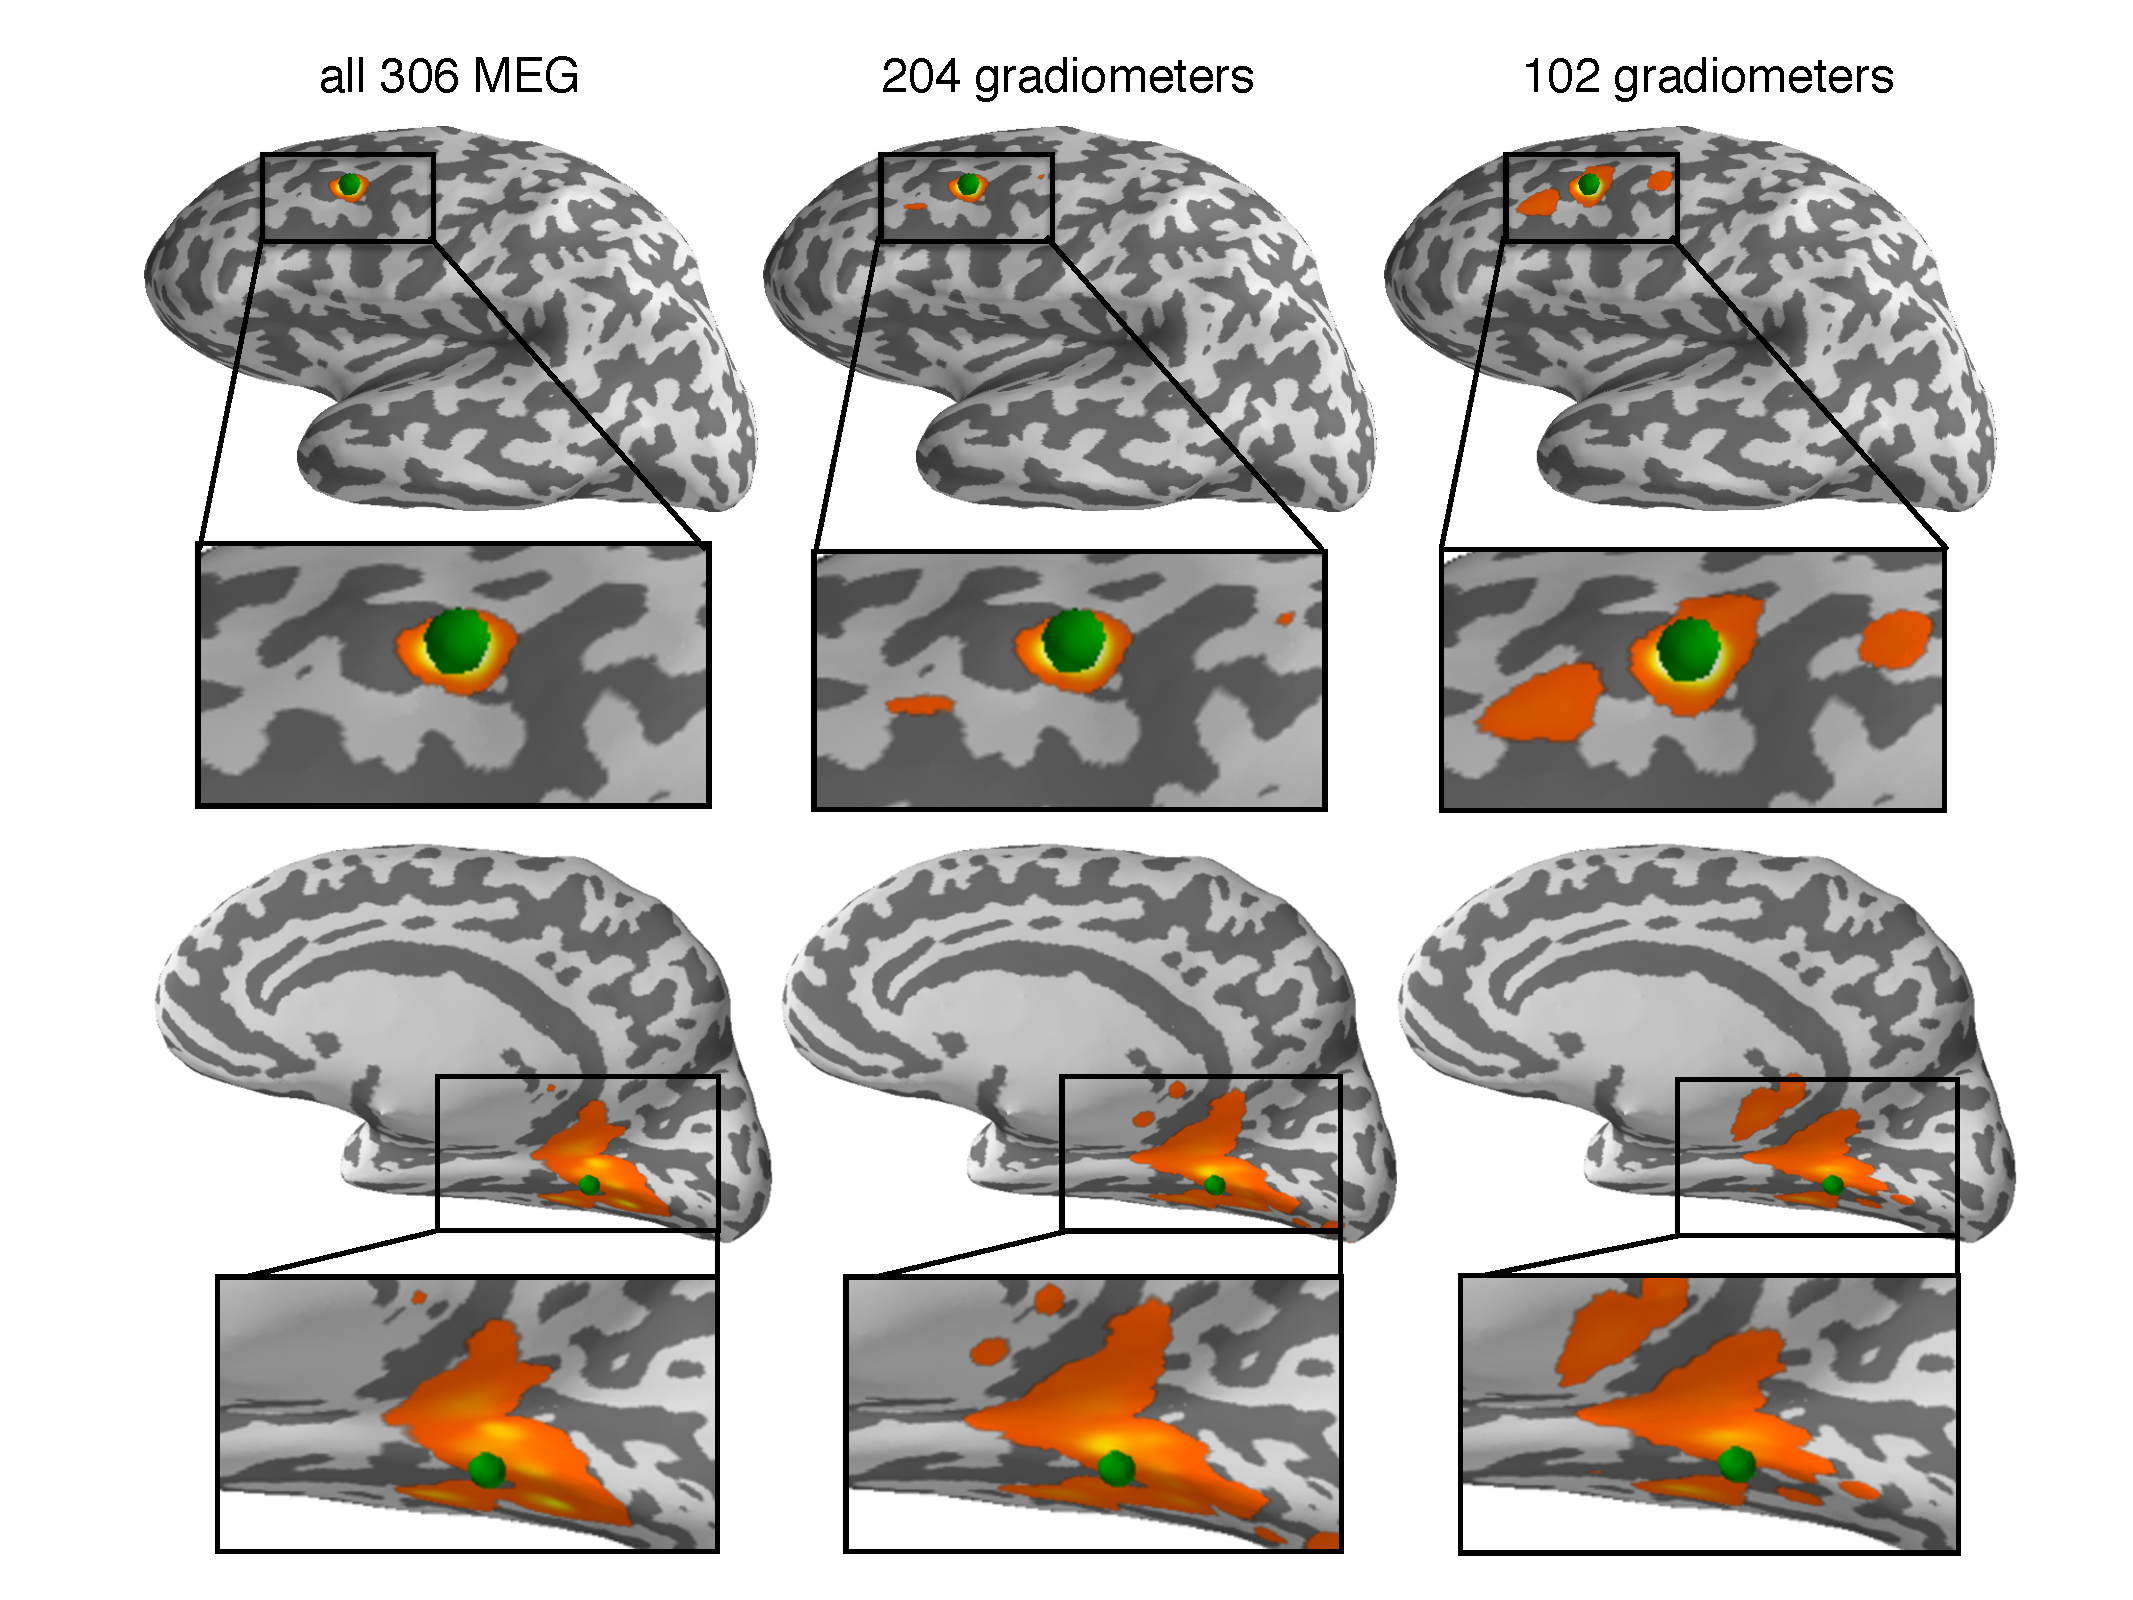
\includegraphics[width=\columnwidth]{hbm/sample_simulated_heat_maps}%
		\end{minipage}
		\begin{minipage}{0.09\linewidth}
				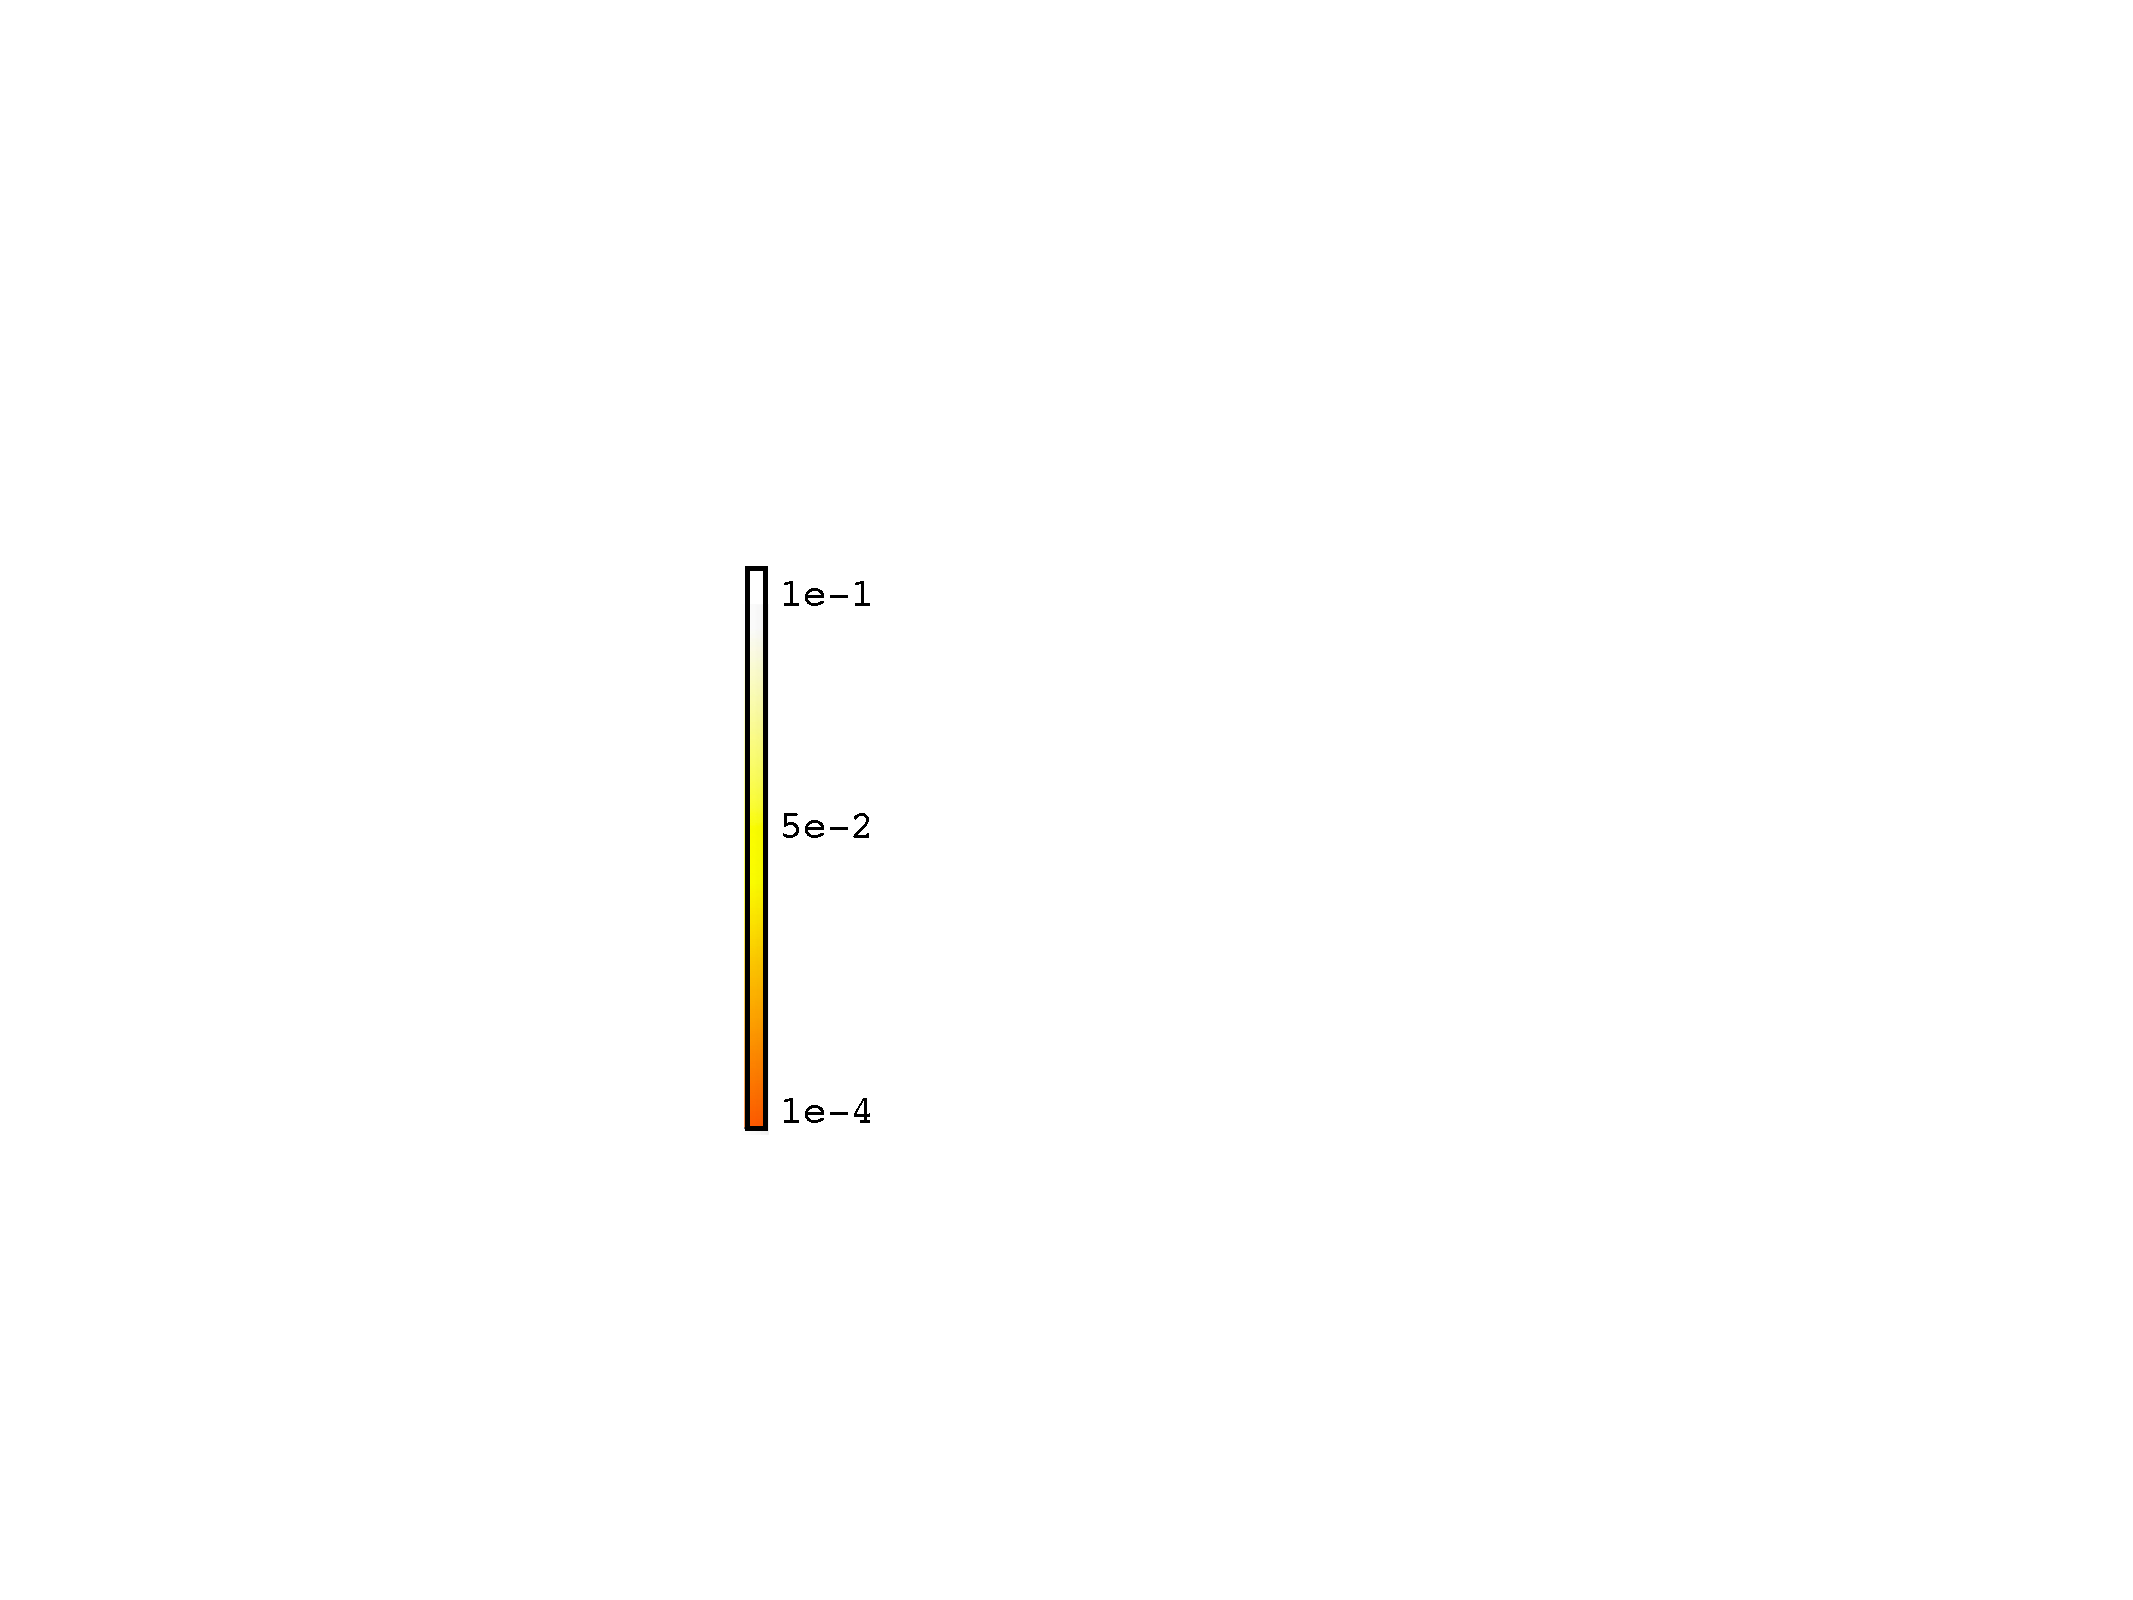
\includegraphics[width=\columnwidth]{hbm/colorbar_heat_maps_key}%
		\end{minipage}
	\end{minipage}
	\caption{The support of the MM results based upon 900 MCMC-based initializations was extracted to build an uncertainty map. The relative frequencies with which each source location was part of the support was computed and plotted on the brain surface together with the two simulated sources (green dots). Each column corresponds to the results for each of the three sensor setups examined. The less the number of sensors and/or the deeper the source is, more uncertain the brain map is.}
	\label{fig:results_simu_heat_maps}
\end{figure}

\subsubsection{Experimental results with MEG auditory and visual data}
We now repeat our analysis with two experimental open datasets. The first one is a recording of auditory evoked fields (MNE sample dataset~\cite{mne-python}). The second one contains visual evoked fields (visual condition of MNE sample dataset) for which source localization is a more difficult task due to the proximity between neural sources. The true nature of the underlying source network is also less clear for this second dataset.

Figure~\ref{fig:hist_real_datasets} shows the equivalent of Figure~\ref{fig:simu_MM_best_MCMC} for both datasets. Again, we see that a lower objective function value can be obtained using MCMC-based initializations. The auditory sample dataset is commonly assumed to be generated by two bilateral focal sources around the auditory cortices in the superior temporal gyrus of the temporal lobe. Due to the superficial nature of these sources and their large distance, the estimation of their position is regarded as a relatively simple task. Indeed, the histogram shows that using MCMC-based initializations does not help a lot to reduce the objective function compared to a uniformly initialized MM solution. In the case of the visual dataset, where several closed-by sources are active, the difference is however quite drastic. The majority of the MCMC-based initializations lead to lower values of the objective function. Looking at the source distribution plots on the brain for both datasets, one can also observe more complex source configurations for the visual data.
% XXX : say here that there is nothing on right hemi for best MCMC?

Next, we repeat the graphical source network analysis from Figure~\ref{fig:results_simu_circular} for the two datasets. Figure~\ref{fig:circular_plots_LAud} shows the results for the auditory dataset and three sensor configurations: all 364 EEG + MEG sensors, all 306 MEG sensors or one over two sensors resulting in 182 EEG + MEG sensors. One can see how adding EEG to MEG sensors reduces the ambiguity of the regression problem. The plots show fewer but more prominent modes, \textit{i.e.} the posterior mass is concentrated on fewer stable source configurations. We also see that the locations of the most prominent modes shift.
This is consistent with results of other studies on EEG-MEG combination \cite{MoStBrHa08,Lu14,AyVoKuHeKuGaHaWeKeRaWoHe14} as EEG is sensitive to some sources that MEG is almost blind to, \textit{e.g.} sources with a strong radial component. If we subsample the EEG+MEG sensors by only using every other location, the ambiguity and spatial spread of the recovered support increases. One can see that there is more activity in the dark green label, which corresponds to a brain area commonly not associated with auditory responses.% On the other hand, there is less activity in the light green label, which marks central areas of the auditory system.
%\ag{what green region do you have in mind?}\felix{Good question, that corresponded to the coloring/parcelation in the old figures. In the new ones, I can't really recall what I wanted to say. Maybe we just drop the sentence and not over-interpret our results?}
The connections between source locations show that none of the found modes really stands out, \textit{i.e.} is found much more often compared to the others. Most of the connections do not occur more than 200 times within the 900 samples, so they are part of the purple background of low frequency connections in the plots.\\
Figure~\ref{fig:circular_plots_LVis} shows the same results for the more complex visual dataset. Compared to the auditory dataset, we see that even with all sensors, the ambiguity of the regression problem seems to be a lot higher compared to the auditory dataset: we see that the posterior mass is distributed among many more source configurations. For the other two sensor configurations, we see similar effects as in the auditory data set. Nevertheless, it can be noticed that the large majority of identified sources with all MCMC initializations are on the right hemisphere. This is consistent with the known functional organisation of the visual cortex. Indeed, in this experimental condition the subject was presented with checker board flashes on the left visual hemifield which is known to primarily project onto the right hemisphere of the cortex.


\begin{figure}[htp]
	\centering
	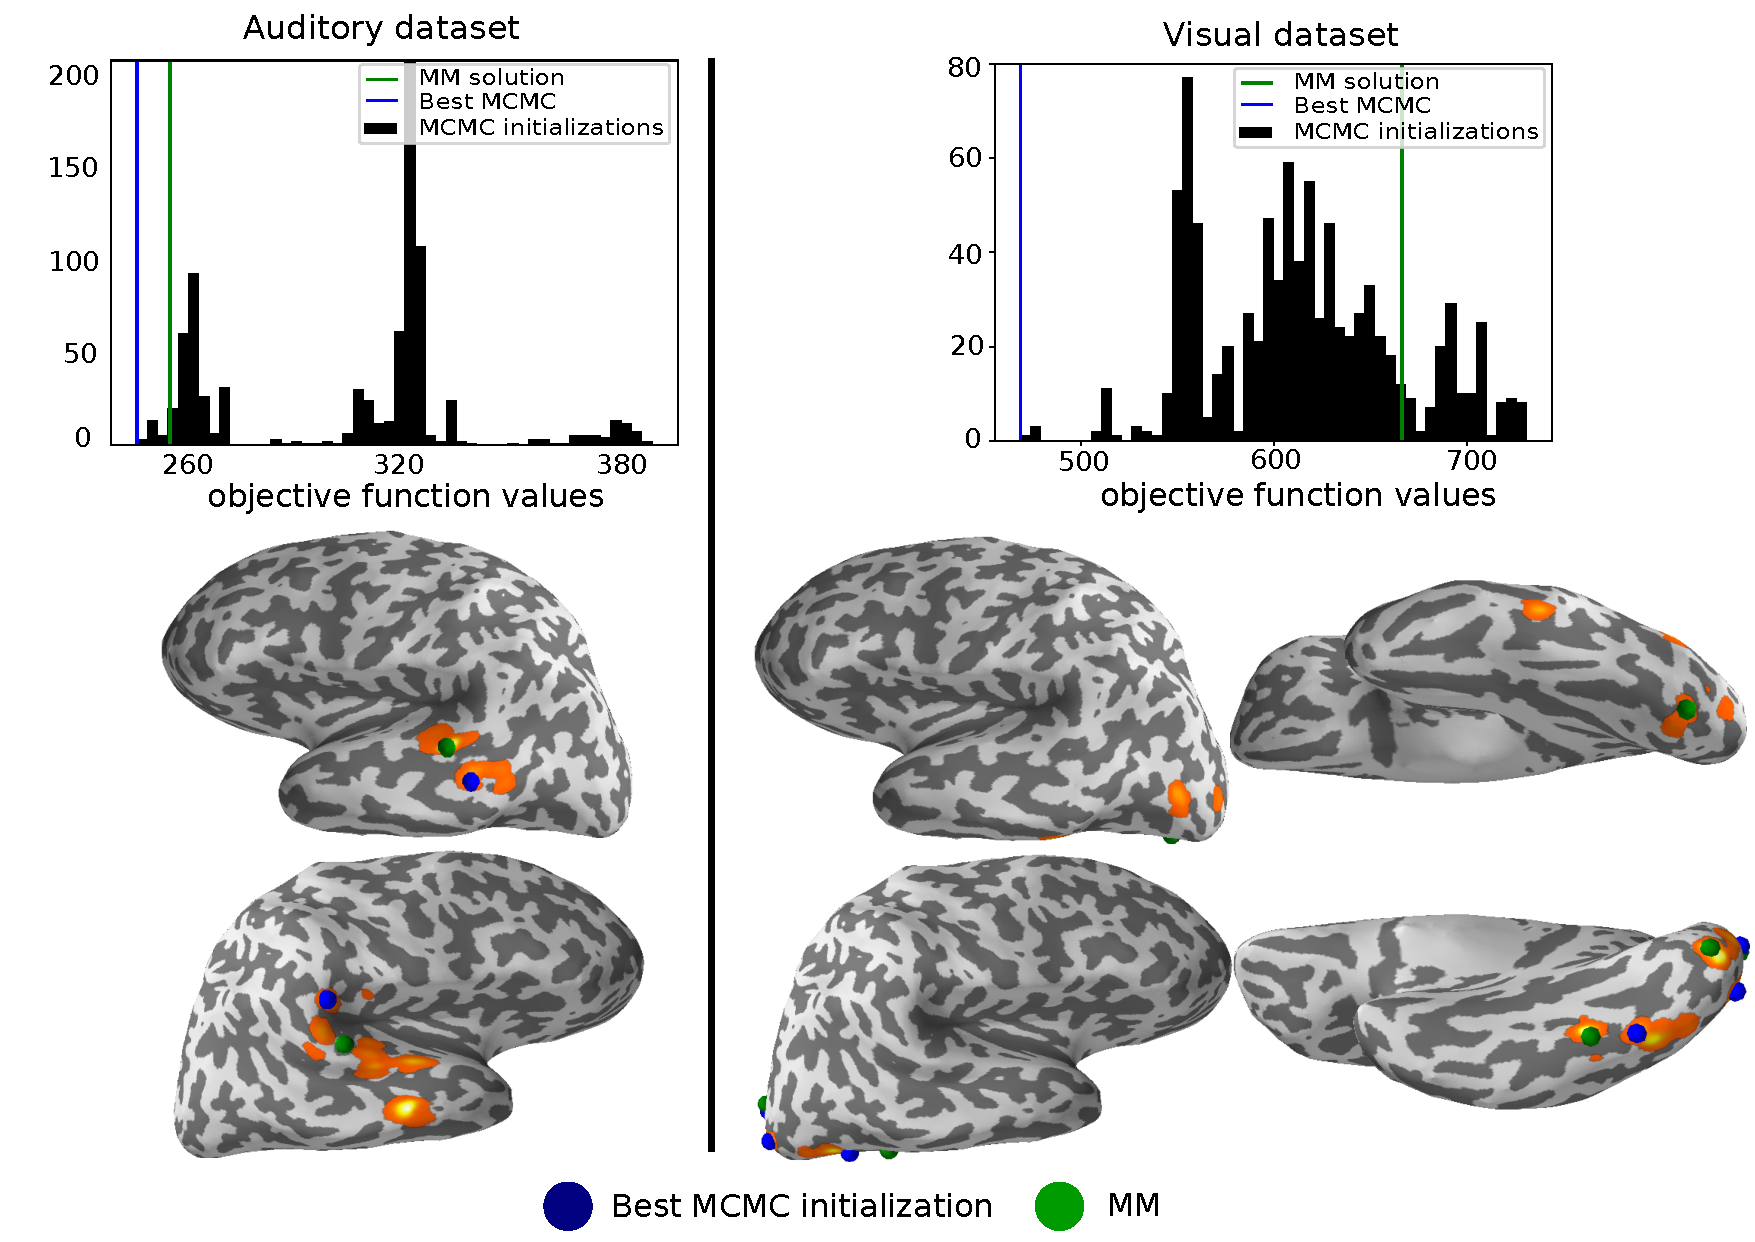
\includegraphics[width=\columnwidth]{hbm/sample_data_hist_vertices}%
	\caption{Histograms of the objective function value for 900 MCMC initializations for auditory and visual datasets (306 MEG sensors). The histogram for the visual dataset shows more MCMC initializations that outperform the uniform one in the MM solution. Under each histogram, these source configurations are shown on the left and right hemisphere.
	}
	\label{fig:hist_real_datasets}
\end{figure}



\begin{figure}[htp]
	\centering
	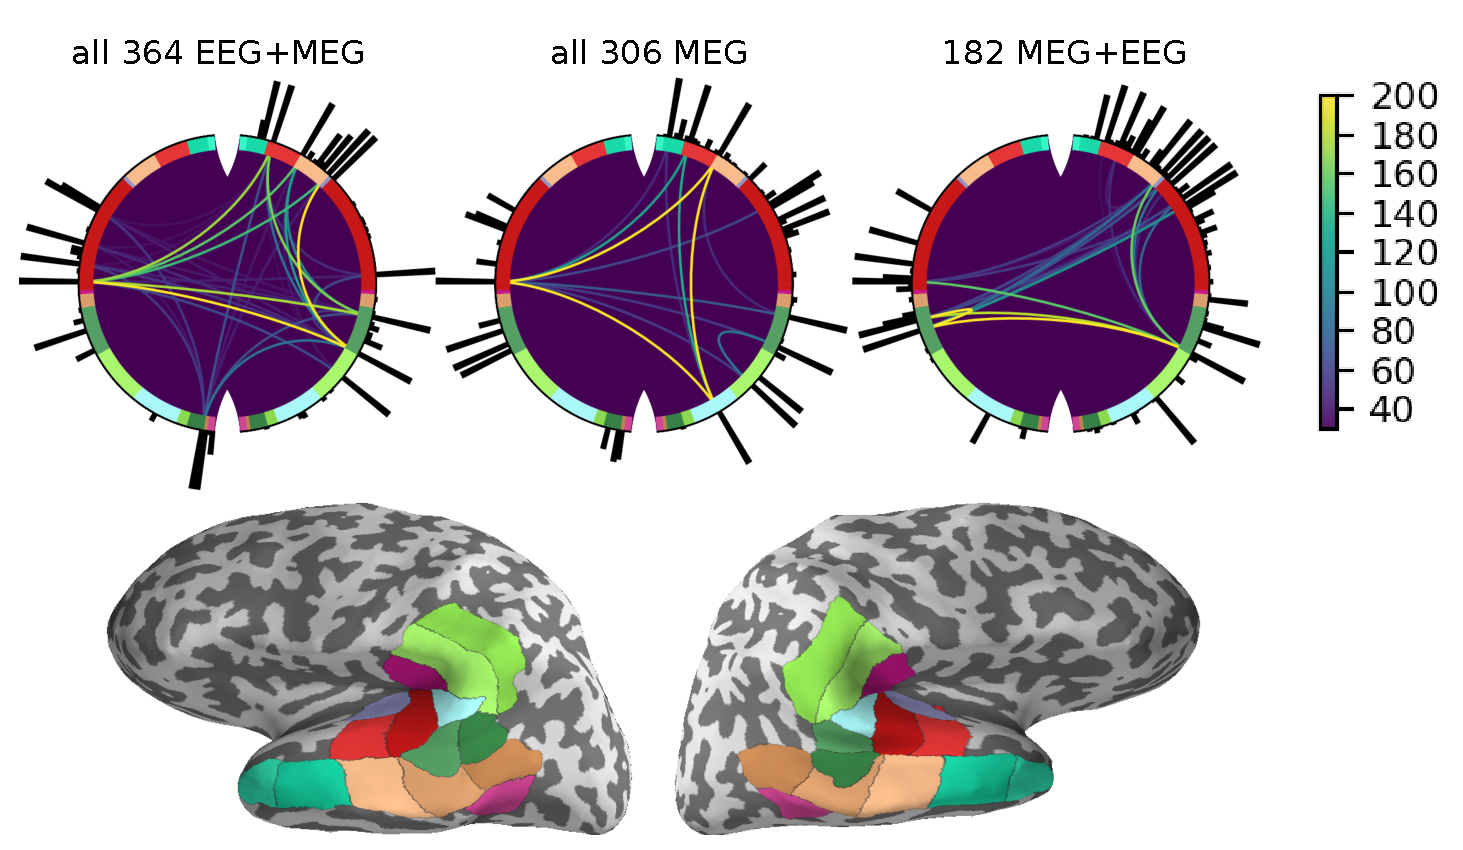
\includegraphics[width=\columnwidth]{hbm/LAud_circular_plots_new}%
	\caption{Source network analysis for auditory data. The figures are constructed in the same way as described in Figure~\ref{fig:results_simu_circular} except that all 900 MCMC initializations are displayed.}
	\label{fig:circular_plots_LAud}
\end{figure}



\begin{figure}[htp]
	\centering
	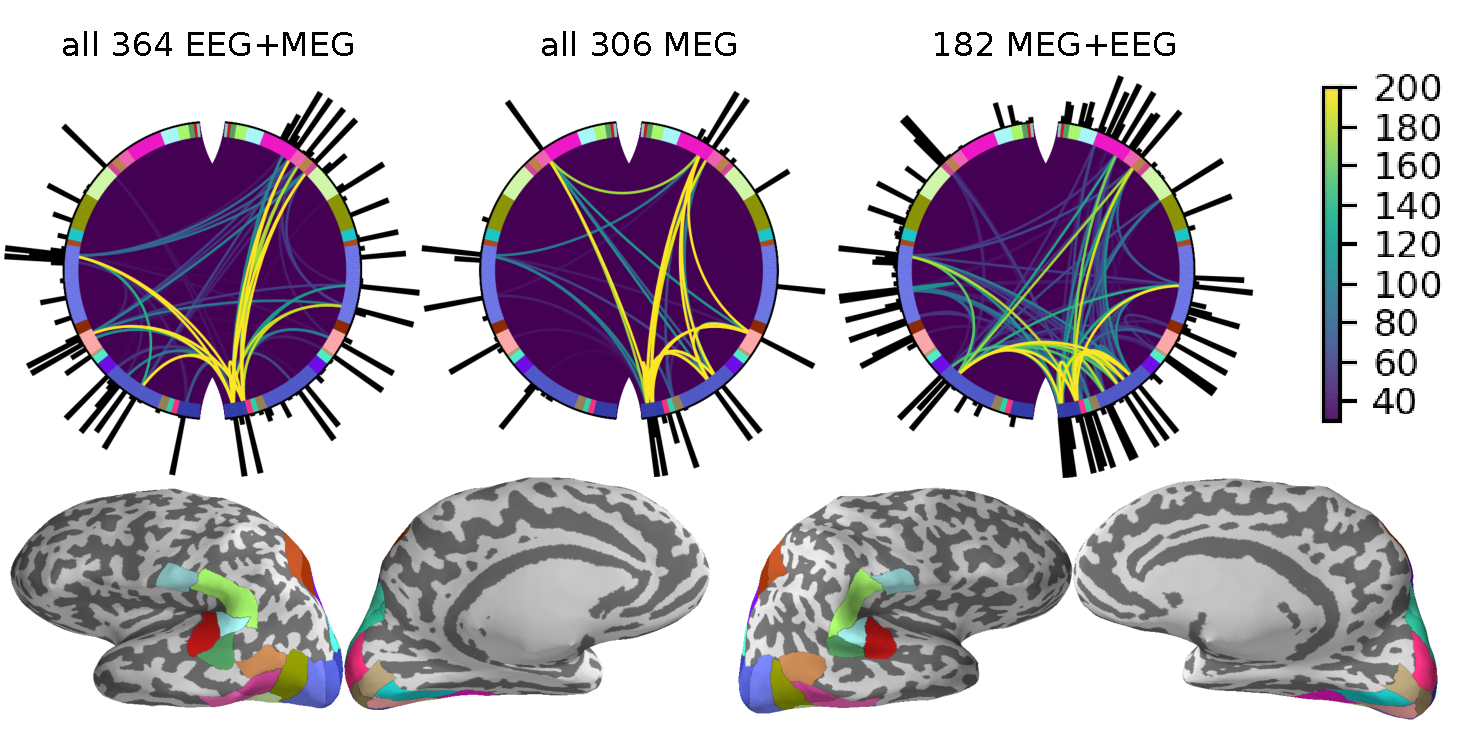
\includegraphics[width=\columnwidth]{hbm/LVis_circular_plots_new}%
	\caption{Source network analysis for visual data. The figures are constructed in the same way as described in Fig.~\ref{fig:results_simu_circular} except that all 900 MCMC initializations are displayed.}
	\label{fig:circular_plots_LVis}
\end{figure}

%----------------Conclusion-----------------------------------------------------------------
\section{Conclusion \& Perspectives}
\label{sec:Dis}
%%%%%%%%%%%%%%%%%%%%%%%%%%%%%%%%%%%%%%%%%%%%%%%%%%%%%%%%%%%%%%%%%%%%%%%%%%%%%%%
%%%%%%%%%%%%%%%%%%%%%%%%%%%%%%%%%%%%%%%%%%%%%%%%%%%%%%%%%%%%%%%%%%%%%%%%%%%%%%%

Scientific literature relying either on frequentist or on Bayesian statistical inference often coexist in many fields ranging from machine learning, inverse problems, signal processing or computational biology.
In this work, we started from an under-determined, ill-conditioned MMV / multi-task regression problem and examined two seemingly unrelated approaches - MM as an optimization technique for tackling non-convex optimization problems arising in frequentist regression, and HBM as a Bayesian prior modeling framework. We showed that one obtains the same algorithms, and therefore the same solutions, when considering some specific choices of models, parameters and inference strategies. In particular the parallel was done between the $\ell_{2,1/2}$-norm regularized regression by MM and the full-MAP estimation for $\ell_{2,1}$ hierarchical priors with specific Gamma hyper-priors. We further showed that this conceptual parallel can be exploited to improve the MM solution by providing well-informed algorithmic initializations.
% , and also to complement the single-point result given by MM - in our case a sparse neuronal source configuration - with a more statistical analysis of the multitude of plausible solutions to the non-convex regression problem.

% For this, we constructed a multi-layered Gibbs sampler for the joint posterior density of our HBM. This sampler has an efficient sub-sampler for $\ell_{2,1}$ priors at its core. We showed that the MCMC scheme is able to quickly jump between the different attractors of the MM scheme by using each sample as an initialization to the MM computation. Each MM computation can then be done with a state-of-the-art convex solver using block coordinate descent techniques and acceleration techniques based on active set strategies.

% As we end up in a different mode with almost every sample, this procedure is well suited to explore different plausible source configurations in more detail. \felix{we don't show this at the moment but it would be easy to add a plot.}
% \textcolor{red}{\textbf{Alternative paragraph:}

For this, we first constructed a multi-layered Gibbs sampler for the joint posterior density of our HBM.
Each sample is then used to initialize the MM step done with a state-of-the-art convex solver using block coordinate
descent techniques and acceleration strategies based on active sets. The sampler used has also an efficient sub-sampler for $\ell_{2,1}$ priors at its core. Despite the multi-modality of the posterior, the MCMC scheme is able to jump rapidely between the different attractors of the MM scheme. Indeed, using each sample as an initialization to the MM computation, one ends up in many different local minima (\textit{cf.} Figure~\ref{fig:hist_real_datasets}, Figure~\ref{fig:circular_plots_LVis}). 
Therefore, this procedure allows us to reveal and explore different plausible source configurations in more details.
% }
% 

Based on this observation, we showcased how one can use the chain of local minima found by MCMC-initialized MM to analyze the variability of the different sparse solutions. Note that this is different from traditional and generic Bayesian uncertainty quantification techniques that use for example covariance estimates or credible sets derived from posterior samples~\cite{szabo2015frequentist}. It is also different from methods developed specifically for parametric M/EEG source localization based on dipole fitting~\cite{Fuchs20041442,Darvas2005355}. These latter approaches cannot easily be transferred to sparse, non-parametric approaches. Using our developed techniques on simulations and actual data, one could observe that uncertainty in MEG/EEG is location specific and also source configuration specific. This is of course well-known by experts in this field, but here we provide a computational approach to visualize it and quantify it.
This is an important incentive to develop such automated, data-dependent methods to quantify uncertainties in the context of MEG/EEG source imaging. In more conventional imaging methods such as Computer Tomography (CT) or \ac{MRI}, the signal originates from weak tissue interaction with strong external fields and the forward operator $\bfG$ depends almost exclusively on the physical properties of the scanner. In this situation, uncertainty is usually distributed in a smooth, well-known way over the image domain. Artifacts as well as real anatomical features are also easy to distinguish for a trained radiologist. The situation for M/EEG is very different. The weak signals originate from endogenous activity, and they are very dependent on dataset specific factors such as source orientation, location and attenuation which all depend on the geometry of the head of the analyzed subject. That is also why the forward matrix $\bfG$ needs to be constructed for each individual patient, after fixing the electrical properties of the head issues, which if wrong, increases the uncertainties.

When considering real data, the source to recover is often poorly understood, especially when it comes to pathological brain activity such as ictal or inter-ictal epileptic activity. In such a situation, providing a single source configuration as a result, together with an ad-hoc uncertainty quantification based on previous studies or acquired expertise, might not be an optimal use of the M/EEG data.
Instead, providing multiple hypotheses together, along with a quantification of their uncertainty, can be more useful. Indeed for applications such as pre-surgical epilepsy diagnosis, where M/EEG recordings are one of several diagnostic modalities, each candidate source configuration can provide some evidence for or against a diagnostic hypothesis that could lead to a surgery decision.
We therefore believe that extending the first steps we took here towards developing a consistent framework for interpreting and quantifying the multitude of potential results of sparse MEG/EEG source reconstruction approaches can have a significant impact on clinical settings.
